% REMEMBER: You must not plagiarise anything in your report. Be extremely careful.


\documentclass{l4proj}

    
%
% put any additional packages here
%

\begin{document}

%==============================================================================
%% METADATA
\title{Redefining a web application for the Robotics Foundations course}
\author{Han Meng Loo}
\date{February 4, 2020}

\maketitle

%==============================================================================
%% ABSTRACT
\begin{abstract}
    The complex lab environment set up process results in a high cognitive load on Robotics Foundation students. The current provided environment, Robotics Foundations Virtual Machine, aims to reduce it. However, the high installation requirements of provided lab environment may lead to a great deal of inconvenience. To solve this problem, Robotics Foundations Web Application has been built to remove any need for students to install and set up an environment before working on the lab exercises. This allows users to concentrate solely on completing their weekly lab exercises. In particular, the web application provides several functionalities, including coding in Jupyter Notebooks, viewing robot visualisations and receiving individual feedback from course coordinators. The evaluation of the web application proved that most project requirements were met and could be highly considered as an alternative platform for students to complete their lab exercises.
\end{abstract}

%==============================================================================
%% ACKNOWLEDGEMENTS
\chapter*{Acknowledgements}
% Enter any acknowledgements here. This is optional; you may leave this blank if you wish,
% or remove the entire chapter
%
% We give thanks to the Gods of LaTeX, who in their eternal graciousness, 
% have granted that this document may compile without errors or overfull hboxes.
%
I would like to thank my supervisor, Dr Gerardo Aragon Camarasa for his invaluable support and guidance throughout the year. I would also like to thank the user evaluation participants and members of the Theia community for their time and input, which was extremely valuable.
%==============================================================================

% EDUCATION REUSE CONSENT FORM
% If you consent to your project being shown to future students for educational purposes
% then insert your name and the date below to sign the education use form that appears in the front of the document. 
% You must explicitly give consent if you wish to do so.
% If you sign, your project may be included in the Hall of Fame if it scores particularly highly.
%
% Please note that you are under no obligation to sign 
% this declaration, but doing so would help future students.
%
\def\consentname {Han Meng Loo} % your full name
\def\consentdate {7 February 2020} % the date you agree
%
\educationalconsent


%==============================================================================
\tableofcontents

%==============================================================================
%% Notes on formatting
%==============================================================================
% The first page, abstract and table of contents are numbered using Roman numerals and are not
% included in the page count. 
%
% From now on pages are numbered
% using Arabic numerals. Therefore, immediately after the first call to \chapter we need the call
% \pagenumbering{arabic} and this should be called once only in the document. 
%
% Do not alter the bibliography style.
%
% The first Chapter should then be on page 1. You are allowed 40 pages for a 40 credit project and 30 pages for a 
% 20 credit report. This includes everything numbered in Arabic numerals (excluding front matter) up
% to but excluding the appendices and bibliography.
%
% You must not alter text size (it is currently 10pt) or alter margins or spacing.
%
%
%==================================================================================================================================
%
% IMPORTANT
% The chapter headings here are **suggestions**. You don't have to follow this model if
% it doesn't fit your project. Every project should have an introduction and conclusion,
% however. 
%
%==================================================================================================================================
\chapter{Introduction}

% reset page numbering. Don't remove this!
\pagenumbering{arabic} 

This chapter will introduce the Robotics Foundation Web Application (RFWA) project, providing the motivation and aims behind the development of the system. In further chapters, this paper will discuss specific areas of the project, background, development, evaluation in detail.
 

\section{Motivation}

Robotics Foundation (RF) (H) is a course provided by the School of Computing Science at the University of Glasgow. The course aims to facilitate students' understanding of core concepts involved in robotic software development, from perception to planning and action. The RF course implements a hands-on learning approach by assigning weekly lab exercises. Students are tasked with prototyping and implementing autonomous robotic systems by making use of a robotic middleware (e.g. Robot Operating System (ROS). 

ROS is officially supported on the Linux operating system (Ubuntu) and it provides libraries and tools to help create and visualise robot systems. Students must have ROS installed on their machine before working on the lab exercises. Students in this course can range from L3 (third years) to L5 (masters students). 

Given a broad range of student levels that can enrol into this course, there will be some students who will be unfamiliar with the Linux operating system. The course provides students with a lab environment, RF Virtual Machine, which students can work on their lab exercises without the need for a Linux OS. The provided environment eliminates the need for Linux OS installation through the use of VirtualBox and Vagrant.

Users intending to set up RF Virtual Machine will be met with system requirements such as having a laptop/PC with 4 core CPU, 16GB RAM and 20GB in free space. The most common laptop RAM size is 8GB, therefore not all students will be able to set up the RF Virtual Machine on their laptop. A student whose system does not meet the requirements can still use the desktops provided in the Boyd Orr Building. Once the RF virtual machine is set up, users have to first download the latest lab before working on them. The buttons on the VirtualBox desktop simplifies the process for which students can download lab files, launch Jupyter notebook, save and restore workspace. From time to time, the RF Virtual Machine will undergo updates. All lab progress in an unsaved workspace will be lost. RF Virtual Machine simplifies the lab environment set up for students, it does not eliminate the process.

\section{Aims}

This paper proposes Robotics Foundation Web Application (RFWA), a web application which aims to reduce the cognitive load of users when dealing with lab environments by facilitating student lab completion and admin lab management all in one centralised application. RFWA should have the core functionalities for students to complete their lab exercises. Students should be able to view all available lab exercises to them, save and download their progress and have access to the necessary tools and features to complete the labs. These include the support of python notebook format and the ability to view robot visualisation through Rviz. Course supervisors (admins) should be able to upload lecture slides, lab exercises and give individual feedback to each student.

Unlike RF Virtual Machine, users will not have to download any files before working on a lab exercise.
RFWA should adopt a minimalist design and be easy to use. The web application should be accessible on any web browser such as Firefox or Chrome, with no compromise of its functionalities on either browser.

\section{Video Demonstration}
 
A demo reel is uploaded on Vimeo which provides visual reference when reading. It can be accessed through, https://vimeo.com/404743981. The password is 'robotics'.

\section{Summary}
This chapter outlined the motivations and aims for this project. The remainder of this paper will discuss how the motivation for RFWA was developed into a working system, and how the aims were met. The paper is structured as follows:

\begin{itemize}
    \item 
    Chapter 2 - \textbf{Background}, introduces tools that needs to be integrated within the system and a review of similar products.
    \item 
    Chapter 3 - \textbf{Requirements}, an outline of the requirements gathering process, from creating user personas and stories to generating a set of functional and non-functional requirements.
    \item 
    Chapter 4 - \textbf{Design}, an overview of the system design followed by why certain design changes were made.
    \item 
    Chapter 5 - \textbf{Implementation}, describes the development progress and implementation details of RFWA.
    \item 
    Chapter 6 - \textbf{Evaluation}, evaluating the system through user evaluation, unit testing and requirements validation.
    \item 
    Chapter 7 - \textbf{Conclusion}, summarises what has been done, an overall reflection on the project and identifying future work.
    
\end{itemize}


%==================================================================================================================================
\chapter{Background}
This chapter will examine the background of the project by investigating the pre-existing services which form the foundations the system is built upon and then look at some existing applications which provides similar functionality and explain why these are not suitable for the problem at hand. 

\section{Project Foundations}

RFWA requires several services implemented to facilitate student lab completion. These services provide functionality such as coding and viewing robot simulations. This section investigates the services which were integrated into RFWA over its development.

\subsection{Online Integrated Development Environment (IDE)}
An online integrated development environment, also known as a Web-based IDE or Cloud IDE is a browser-based IDE that allows for software development. An online IDE can be accessed from a web browser, such as Firefox or Chrome, which allows for a portable work environment

The main advantage of implementing an online IDE is that students of the RF course can dive straight into working on the weekly lab exercises, without the need to set up a development environment. Given that no setup is required, this saves storage space and time compared to installing Ubuntu/ ROS and Vagrant/ VirtualBox

However, an online IDE is not as feature-packed as a traditional IDE, such as the lack of third party marketplace extensions. Nevertheless, the core features such as compiling and running code and displaying errors should be provided.

\subsection{Robot Operating System (ROS)}

The \cite{ROS} is a flexible open-source framework for writing robot software. It is a collection of tools, libraries, and conventions that aim to simplify the task of creating complex and robust robot behaviour across a wide variety of robotic platforms. 

Before ROS, roboticists often had to reinvent the wheel and write a whole software system from scratch. With ROS, it is easier to reuse components from other robotic systems, including the ones that other people wrote. For example, one laboratory might have experts in mapping indoor environments and could contribute a world-class system for producing maps. Another group might have experts at using maps to navigate, and yet another group might have discovered a computer vision approach that works well for recognizing small objects in clutter. ROS was designed specifically for groups like these to collaborate and build upon each other's work. This is implemented through the use of a publisher and subscriber nodes. These nodes communicate with one another without having to have direct knowledge of the other nodes in the system. As ROS is the framework of choice for the RF course, therefore, the project has to be developed in which ensures that ROS can be executed within it.

\subsection{Robot Visualisation (RViz)}

\cite{Rviz}, an abbreviation for ROS visualization, is a 3D visualisation tool for ROS. Rviz allows the user to view the simulated robot model, log and replay sensor information such as cameras. By visualising what the robot is seeing, thinking, and doing, the user can obtain feedback and debug a robot application from sensor inputs to its desired actions. Rviz plays a vital role in aiding student lab completion, therefore, it must be integrated into the workspace.

\subsection {Gazebo}

Robot simulation is an essential tool in every roboticist's toolbox. \cite{Gazebo} is a simulator which makes it possible to rapidly test robots using user-defined realistic scenarios by adding obstacles or environmental properties such as gravity and inertia. Gazebo offers the ability to accurately and efficiently simulate populations of robots in complex, indoor, outdoor and dangerous environment without any harm to the robot. It is also faster to run a simulator instead of starting the whole scenario on a real robot. Like Rviz, Gazebo plays a vital role in aiding student lab completion, therefore, it must be integrated into the workspace.

\subsection{Virtual Network Computing (VNC)}
Virtual Network Computing is a graphical client-server desktop-sharing system that uses the Remote Frame Buffer protocol to remotely control another computer. It transmits the keyboard and mouse events from one computer to another, relaying the graphical-screen updates back in the other direction, over a network.

\begin{figure}[h]
    \centering
    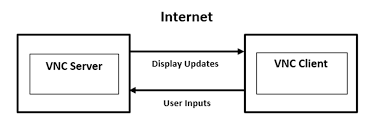
\includegraphics{images/vnc_image.png}
    \caption{Interaction between VNC client(user)-server.}
    \label{fig:vnc_diagram}
\end{figure}

\subsection{IPython}

IPython, (.ipynb) file format, is a powerful interactive Python interpreter that is more interactive compared to the standard interpreter. IPython provides a rich toolkit to help users make the most out of using Python. IPython provides the following features:

\begin{itemize}
    \item 
    Interactive shells (terminal and Qt-based).
    \item 
    A browser-based notebook interface with support for code, text, mathematical expressions, inline plots and other media.
    \item 
    Support for interactive data visualization and the use of GUI toolkits.
    \item 
    Flexible, embeddable interpreters to load into one's projects.
    \item 
    Tools for parallel computing.
\end{itemize}

IPython itself is focused on interactive Python, part of which is providing a Python kernel for other Project Jupyter products (Jupyter Notebook and JupyterLab).

\section{Related Products}
There are several existing online coding platforms. This section intends to identify any strengths or weaknesses in each product and discuss how it has influenced the project.

\subsection{Jupyter Notebook}

\cite{JupyterNotebook} (formerly IPython Notebooks) is an open-source server-client web application that supports multiple language kernels, including IPython. Jupyter Notebooks are experiencing immense success in recent years, it is being applied in education and research fields such as computer vision and machine learning. Given its popularity, some students in the course should already be familiar with its environment (e.g code execution, comment structure etc).  Jupyter Notebook provides excellent support for IPython kernels, but it needs to be paired with other tools as it does not have inbuilt support for RViz and Gazebo.

\subsection{Previous L4 Project}
The previous L4 project, \cite{previousl4} is a web application which aims to solve a similar problem at hand. The project was an online IDE deployed through a \cite{Docker} container which controls the interactions between the application and the client. \cite{Supervisor} is a system that was implemented to launch, maintain and kill tools on UNIX-like operating systems. A wide variety of tools were implemented in the workspace to aid student lab completion. 

At the end of L3, the first project meeting took place which outlined relevant summer preparation work and project plans. The initial plan for this project to improve upon the previous L4 project based on feedback received through user evaluation and the project supervisor. These included wider browser support apart from Google Chrome, improving the reliability of the workspace terminal and user interface improvements such as dark theme support. 

However, the plan was later dropped in the first semester meeting with project supervisor as there was a change in deployment method due to security issues. Furthermore, developing a new web application provided more flexibility to the new system as it was not bounded to the compatibility requirements of the existing framework and tools used. Nevertheless, the previous L4 project provided excellent suggestions to some of the tools which were later used during project development.

\subsection{Gitpod}

\cite{Gitpod} is an online IDE for GitHub and GitLab that launches ready-to-code development environments for any project with a single click. Users can click on the Gitpod button on the repository page or prefixing any GitHub URL with gitpod.io/\# to begin working on a repository in Gitpod. The Gitpod button is a browser extension (Chrome or Firefox) which is available on the extension marketplace of respective browsers. Gitpod allows coding in several programming languages including Python. Students of the RF course will have to upload their lab exercises as a repository before working on them on Gitpod and set up is required for a Jupyter Notebook server. Although these steps are easy to complete, students will spend an unnecessary amount of time on set up over the duration of the RF course.

Like Jupyter notebook, the main issue would be the absence of Gazebo and Rviz. Without these, robot visualisation and debugging would be harder for students and will impact their learning progress. Furthermore, course coordinators might want students to privatise their repository to prevent code copying. The ability to work on private repositories on Gitpod is only accessible by paying users which starts at 8 \euro  per month. 

\subsection{ROS Development Studio (ROSDS)}

As a beginner in robotics, one has to have ROS installed and understand the required tools and steps to create and run robot simulations. Furthermore, complex concepts and terminology may put off beginners intending to start using ROS. \cite{ROSDS} plans to overcome this by providing ready-to-code environments with the tools required. To help beginners get started, ROSDS contains extensive documentation and a large set of samples and tutorials that illustrate how to program and test robots. Users who are not satisfied with the sample projects can create their own and share via a simple link. ROSDS projects can be shared and reproduced on any computer without requiring any installation. On top of that, everything is wrapped up in a user-friendly environment. This solves the current problem at hand, course coordinators can create custom ROS projects which meets the learning outcomes of the lab exercises.

The main issue would be the cost associated with ROSDS. Student lab projects should be private to prevent code copying. The ability to create private projects is only available to users signed up with the "developer" tier package, which costs 9 \euro per month. Hardware limitations will drive the cost up as well, the "free" and "developer" tier package only allows for 8 hours of development per month, which may be insufficient for students to complete their labs. In both packages, the hardware specifications are restricted to 2 core CPU and 8GB RAM. If students are unable to view their robot simulations, their learning progress might be impacted. ROSDS does provide extra computing power and time, starting from 14 \euro (10 hours with 8 core CPU and 16GB RAM). The university and RF course could be looking at a yearly recurring cost of 2300 \euro for a class of 100 students, which is not feasible.

\subsection{JupyterLab}

\cite{JupyterLab} is an interactive development environment for working with notebooks, code and data. Most importantly, JupyterLab has full support for Jupyter notebooks. JupyterLab offers users an IDE-like experience by providing common IDE features such as text editors, terminals, data file viewers, and other custom components side by side with notebooks in a tabbed work area. JupyterLab is built on top of an extension system that enables users to customize and enhance JupyterLab by installing additional extensions. Users can develop extensions to meet custom requirements. Like Jupyter Notebook, JupyterLab has IPython kernels but additional tools and extensions are needed to allow users to view robotic visualisations. 

\subsection{Chapter Summary}

This chapter reviewed multiple existing products, both academic and commercial, and how each of these influenced the system in some way. It can be pointed out that these products are well-developed, but they do not solve the problem at hand. This can be due to service limitations or pricing options. In the following chapters, the proposed system, influenced by the design and implementation techniques of these related products, will attempt to integrate technologies outlined in the project foundations, to meet project requirements.



%==================================================================================================================================
\chapter{Requirements}
This chapter will outline the functional and non-functional requirements which the system has to fulfil. Requirements gathering was done at the beginning of the project, these are revised and updated after each iteration. 

\section{Requirements Gathering}
Requirements for this project were gathered from the supervisor and evaluating the received feedback in the previous L4 project. After the first meeting with the project supervisor, a basic set of requirements were drafted. This provided great depth on what was expected from the RFWA. Requirements gathered were categorised using the \cite{Moscow}.

\subsection{User Personas}

\textbf{Robert}, a Level 3 student Robotics Foundation Student. He wants the ability to receive and complete his weekly lab exercises all in one place. He is frustrated that he has to log in to moodle does not want to sign in to multiple services to complete his lab. 

\textbf{Timothy}, a robotics foundations student, lost his laptop. Timothy was given a temporary laptop and does not want to load it with foreign files such as installing Vagrant and VirtualBox to complete his lab exercise due next week. Timothy would like to work on the labs without the need to install any additional files. 

\textbf{James}, a robotics foundation student who lives far away from the University. He usually works on his lab exercises on the provided lab environments in the LV 10 computing lab in the Boyd Orr Building. He does not want to take a 2-hour train ride every weekend to the University to complete his lab exercises, restricted by the location which he can complete his lab exercises.  He would much prefer the ability to work on his lab exercise anywhere, from home or his favourite coffee shop.

\textbf{Emma}, a robotics foundation student is frustrated that the lab set up requirements include a 16gb ram requirements. She wishes that the requirements are lower or none at all so that she can work on her laptop

\textbf{Blake}, a robotics foundation course coordinator at the University of Glasgow. He wants a lab environment which some students might be familiar with. He believes that a familiar development environment will increase the productivity of the users.

\subsection{User Stories}
User stories were derived from user personas which identified what features RFWA should provide.

\textbf{Student (RFWA user):}

Iteration 1:

\begin{itemize}
    \item
    \emph{As a} student, \emph{I want} to be able to complete my lab work on an online IDE, \emph{So that} I can avoid any issues arising from setting up a development environment on my laptop.
    \item
    \emph{As a} student, \emph{I want} to be able to save my current lab progress to continue later, \emph{So that} I do not have to recode my previous code and save time.
    \item
    \emph{As a} student, \emph{I want} an online IDE which works on any OS and browser, \emph{So that} I can use my preferred browser + OS and do my weekly lab exercise.
    \item
    \emph{As a} student, \emph{I want} the ability to chat with my peers, \emph{So that} I can provide and receive help outside lab hours.
    \item
    \emph{As a} student, \emph{I want} the ability to view lecture slides, \emph{So that} I do not have to log into Moodle to view lecture slides.
    \item
    \emph{As a} student, \emph{I want} the ability to receive feedback, \emph{So that} I am aware of how I am performing in this course and improve myself.
    \item
    \emph{As a} student, \emph{I want} a development environment which I am familiar with, \emph{So that} I can save time by dive straight into coding without the need to familiarise myself first.
\end{itemize}

Iteration 2:

\begin{itemize}
    \item
    \emph{As a} student, \emph{I want} to be able to switch lab workspaces seamlessly, \emph{So that} I dedicate more time to completing the labs.
\end{itemize}

Iteration 3:

\begin{itemize}
    \item
    \emph{As a} student, \emph{I want} to be able to update my lab completion status, \emph{So that} I am aware of the labs that I have yet to complete.
    \item
    \emph{As a} student, \emph{I want} to be able to view upcoming datelines on a familiar format like SoCS online, \emph{So that} I am aware of all upcoming datelines.
    \item
    \emph{As a} student, \emph{I want} to be able to download my lab progress, \emph{So that} I can view it in the future.
    \item
    \emph{As a} student, \emph{I want} to receive reminders when I have yet to complete a lab that is due soon, \emph{So that} I can complete and hand it in before the deadline.
\end{itemize}

\textbf{Course coordinator (RFWA admin):}

Iteration 1:

\begin{itemize}
    \item
    \emph{As a} course coordinator, \emph{I want} an online IDE app for students to complete their lab work, \emph{So that} I can save time by not having to look into student development environment setup issues.
    \item
    \emph{As a} course coordinator, \emph{I want} a system for which students can submit their lab exercises for grading, \emph{So that} I can manage them easily.
    \item
    \emph{As a} course coordinator, \emph{I want} some measures to prevent lab copying, \emph{So that} students can not cheat.
\end{itemize}

Iteration 2:

\begin{itemize}
    \item
    \emph{As a} course coordinator, \emph{I want} to be able to provide individual feedback to students, \emph{So that} they can work on suggested improvements in the next lab.
    \item
    \emph{As a} course coordinator, \emph{I want} the ability to get track cumulative time spend on each lab by students, \emph{So that} I can gauge the lab difficulty and make necessary changes if the lab is too hard.
\end{itemize}

Iteration 3:

\begin{itemize}
    \item
    \emph{As a} course coordinator, \emph{I want} to be able to view the individual feedback which I provided to students, \emph{So that} I can change them if there are any mistakes.
\end{itemize}


\section{Functional Requirements}

Once the requirement gathering process was completed, a set of functional requirements could then be generated. Functional requirements define the functionality of the software, which have to be developed so that the users could easily perform their tasks up to the intended requirements. These requirements are categorised based on the MoSCoW method, which prioritises requirements based on the following categories.

\begin{itemize}
    \item
    \emph{Must Have} - These are things that the system simply must have or it will be useless or unusable. Must requirements will form the central basis of the project plan as these requirements must be met.
    \item
    \emph{Should Have} - This is a secondary requirement that, while not critical to the project, should be included in the overall build. It might be possible to leave a should requirement out, but only if there is another way of doing what is expected.
    \item
    \emph{Could Have} - Could requirements are things that have no impact on the function of the system, but which might, for example, save time in the operation of the program at a later date.
    \item
    \emph{Won't Have} - Requirements the system could have added further down the line to further increase functionality, however, they will not be developed in this delivery.
\end{itemize}

Like the user stories above, the functional requirements have been separated into user types. This allowed a single user type to be focused on at one time throughout development. Admins should have similar access as a standard user would. The requirements are listed below, categorised based on their importance. 

\subsection {Must Have}

User:
\begin{itemize}
    \item 
    Users must be able to create an account.
    \item
    Users must be able to complete their lab exercises through the system.
    \item
    Users must be able to code in Jupyter Notebook.
    \item
    Users must be able to view robotic visualisation.
    \item
    Users must be able to switch lab workspaces easily.
\end{itemize}

Admin:

\begin{itemize}
    \item 
    Admin must be able to upload labs.
    \item
    Admin must be able to upload lecture slides.
    \item
    Admin must be able to delete uploaded labs.
     \item
    Admin must be able to delete lecture slides.
     \item
    Admin must be able to unzip uploaded labs.
    \item
    Admin must be able to specify the due date for each lab.
\end{itemize}

\subsection {Should Have}

User:

\begin{itemize}
    \item 
    Users should be able to receive individual feedback.
    \item
    Users should be able to download their code.
    \item
    Users should be able to receive notifications on incomplete labs which are due soon.
\end{itemize}

Admin:

\begin{itemize}
    \item 
    Admin should be able to update details on uploaded contents.
    \item
    Admin should be able to provide individual feedback to student users.
    \item
    Admin should be able to view students username's to assign feedback.
\end{itemize}

\subsection {Could Have}

General:

\begin{itemize}
    \item 
    The web app could have a calendar which displays upcoming due dates to the user.
    \item 
    The web app could have a task manager which users can update the lab completion status.
\end{itemize}

User:

\begin{itemize}
    \item 
    Users could be able to customise the theme on the web app.
\end{itemize}

Admin:

\begin{itemize}
    \item 
    Admin could be able to view the total time spent by all users on each lab.
\end{itemize}

\subsection {Won't Have}

User:

\begin{itemize}
    \item 
    Users won't be able to submit their lab exercises through the system.
    \item
    Users won't be able to sign in and register using their university email "@student.gla.ac.uk".
    \item
    Users won't be able to chat with other users on the system.
\end{itemize}

Admin:

\begin{itemize}
    \item 
    Admin wont be able to view stats of individual users.
\end{itemize}

\section{Non-Functional Requirements}

A set of non-functional requirements were also generated before any further development took place. Non-functional requirements are equally as important as they describe how the system works.

\begin{itemize}
    \item 
    The system must be easy to use.
    \item 
    The system must be accessible by all parties involved in the RF course.
    \item 
    All users must be able to complete their lab without any installation.
    \item 
    Student users must not be able to modify labs, lecture slide and feedback.
    \item
    Analytical data must not be invasive.
\end{itemize}

%==================================================================================================================================
\chapter{Design}

This chapter will outline the design of the system, starting with its architecture. The user interface for the system will also be discussed. Finally, the chapter will go on and examine the design and technology changes throughout development.

\section{System Architecture}

\begin{figure}[h]
    \centering
    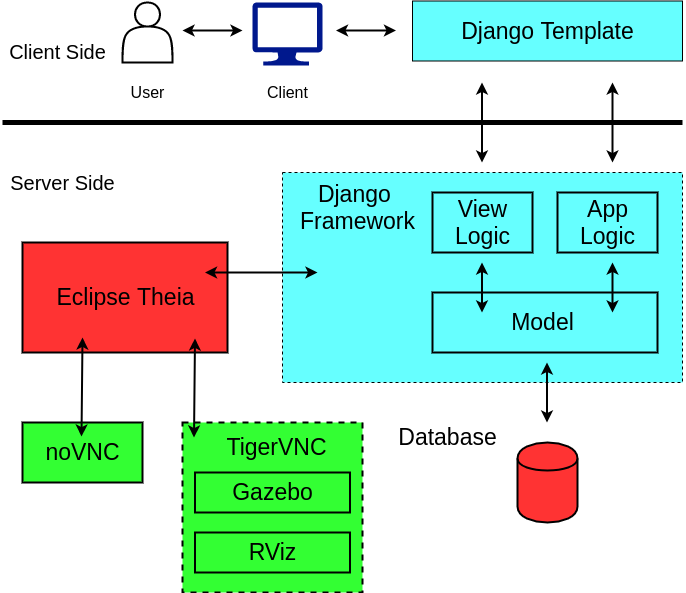
\includegraphics[scale=0.4]{images/system_architecture.png}
    \caption{A full system diagram which describes the connections between each component of RFWA.}
\end{figure}

A system architecture is a conceptual model that defines the structure in a system. This is useful in determining the interaction between the various components of the web application and provides a better understanding. In RFWA, users interact with the web application through a client (web browser). The server receives interaction (clicks) and passes on the appropriate view back to the Django Template. The corresponding HTML, CSS, JavaScript is then rendered to the user. 

Django implements a Model-View-Template (MVT) pattern. MVT is a collection of three important components, Model, View and Template. The Model helps to handle database. It is a data access layer which handles the data. The Template is a presentation layer which handles User Interface part completely. The View is used to execute the application logic and interact with a model to carry data and renders a template. Although Django follows MVC pattern but maintains it's own conventions. So, control is handled by the framework itself.

It was outlined by project supervisor that RFWA will be developed with 1 user in mind, such that users in RFWA will not interact with one another. Project development was not heavily considered as project supervisor stated that the deployment would be handled by him. The project was only deployed locally for development and conducting user evaluation. Implementation of tools and technologies were discussed beforehand to ensure they are supported during deployment.

\section{User Interface}

User Interface (UI) is one of the most crucial aspects of any application. Having a good UI creates fewer problems, increases user involvement and creates a strong link between users and the application. The system must be intuitive and easy to use by untrained users. With that in mind, here are some aspects which should be considered and implemented:

\begin{itemize}
    \item 
    Easily navigable menus - Fancy layouts and multiple interface patterns may be tempting, but it may make site navigation more difficult for users. Every part of RFWA should be clearly labelled on the navigation menu and placed strategically for the users. 
    \item 
    Simplistic design - By sticking with a simple design, RFWA users can identify the services offered without confusion. Complicated designs may look phenomenal, but it’s likely to cloud the system’s underlying purpose.
    \item 
    Consistency - Reusing common elements (e.g. same themes, button attributes) creates a sense of familiarity across RFWA which allows users to understand patterns and learn how the system works.
    \item 
    Communication - Users should be notified about their actions. Therefore RFWA must be able to communicate effectively with the users. These include error messages (e.g. admin failing to add a lab exercise), execution messages (e.g. RFWA downloading user’s lab for storage) and content messages (e.g. if there are no lab uploaded). These messages should be short and easy to understand.
    
\end{itemize}

\section{Initial Prototyping using Wireframes}
Before implementation, low-fidelity visual representation of RFWA's layout design was created. These wireframes illustrate the understanding of the project supervisor's vision of RFWA. Being a prototype, these were easy to make, discard and adapt based on the feedback received.

Initially, 2 sets of wireframes were drafted. The first set was a simple web application with 2 pages, 1 for choosing the labs and the other for working on the labs (workspace page). The second set provided RFWA with more functionalities such as the ability to view lecture slides, receive feedback and a user summary page. After further discussions, it was agreed upon to develop based on the second wireframe set as it meets more functional requirements. The wireframe for the workspace page was inspired by ROS Development Studio and previous L4 project. It allowed users to identify and select tools needed while providing flexibility, the ability to move tool windows around. The tools were located at the top of the web page, which is similar to a standard IDE. 

\section {Design Changes}

There are multiple reasons for design changes throughout the project timeline. These can result from changes in project requirements, service limitations and changes in implemented technologies. Most design changes took place during the first iteration as changing tools and frameworks mid iteration would mean past development efforts using older tools and frameworks would be wasted. The subsections below intend to highlight several design changes throughout the project development. Justifications on technology changes will be provided in the next section.

\subsection{Registration Page (Iteration 1)} 

For authentication purposes, users had to enter their student email when registering with RFWA. This was to ensure that each user was using his student id so that feedbacks and grades can be assigned correctly. This was later dropped as sending an email to student's email address required the RFWA to be registered and granted necessary permissions by the university's Outlook365 system administrator. 

\subsection{Workspace Layout (Iteration 1)}

Inspired by the workspace layout in ROS Development Studio and the previous L4 project, the workspace should be a combination of multiple web technologies. These included Jupyter Notebook for python notebook support and xterm.js for in-browser terminal support. However, the project supervisor suggested extending an online IDE, an approach which was not tried in the previous L4 project. By extending an online IDE, a significant amount of time would be saved as certain features in an online IDE could be reused in RFWA to meet core requirements. Eclipse Theia was the framework of choice and implemented in the workspace page shown below.

 Users can toggle the navigation sidebar (Toggle Menu button in blue) at the top right and scroll down to minimise the side and top bar in the workspace page. This allows RFWA to provide a full-screen experience to users which is similar to a traditional desktop IDE.  Furthermore, this provides more screen real estate which can increase student's productivity when working on the lab. The implementation of Eclipse Theia into the workspace page will be discussed in the next chapter.
 
 \begin{figure}[h]
    \centering
    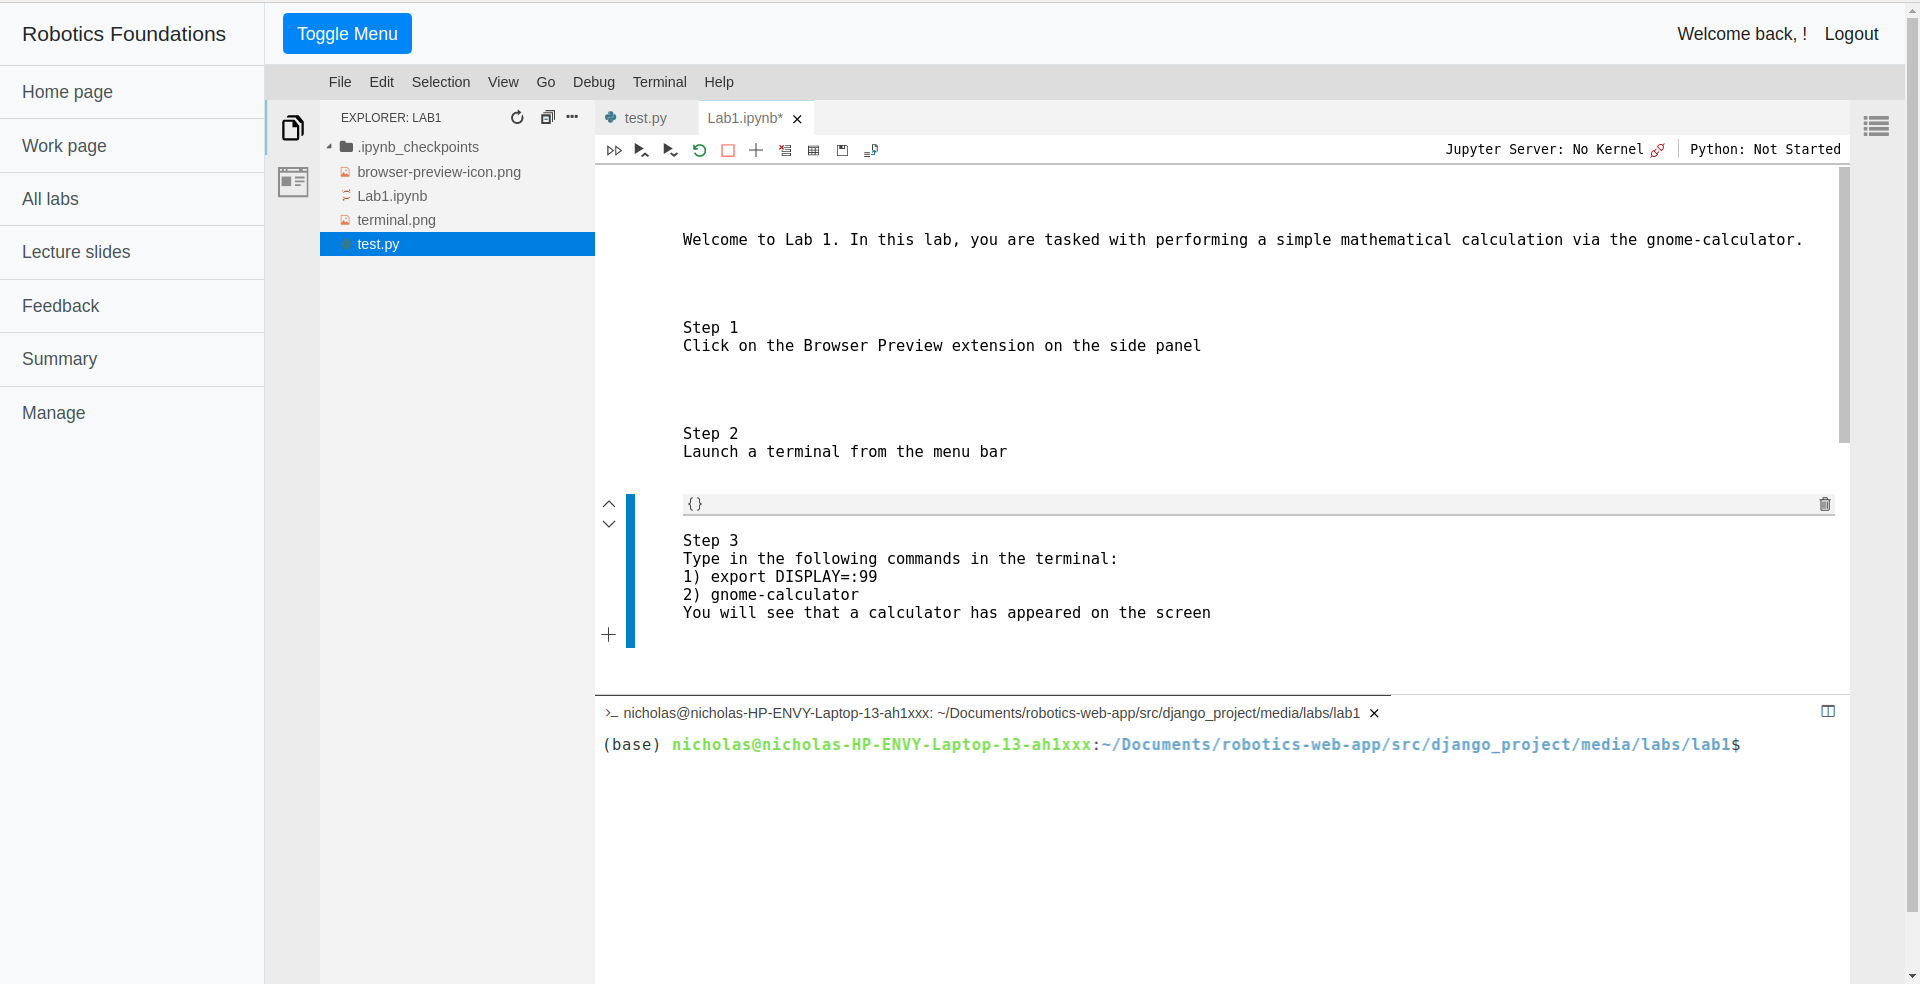
\includegraphics[scale=0.2]{images/workspace_design.png}
    \caption{RFWA's workspace with the user evaluation files.}
    \label{fig:workspace_page}
\end{figure}

\subsection{Admin Manage Page (Iteration 1)}

Django web development framework provided an admin interface which allowed RF course coordinators to manage contents on RFWA. However, the default admin interface is not accessible on the web application. Project supervisor requested an admin interface to be embedded within RFWA which allowed for easier management of RFWA contents. Here, contents are separated into categories (Labs, Slides, Feedback and Users). This allows admins to manage the site effectively as it reduces the chance of any confusion (e.g. lab and slide files having the same name). A screenshot of the admin management page is shown below.

\begin{figure}[h]
    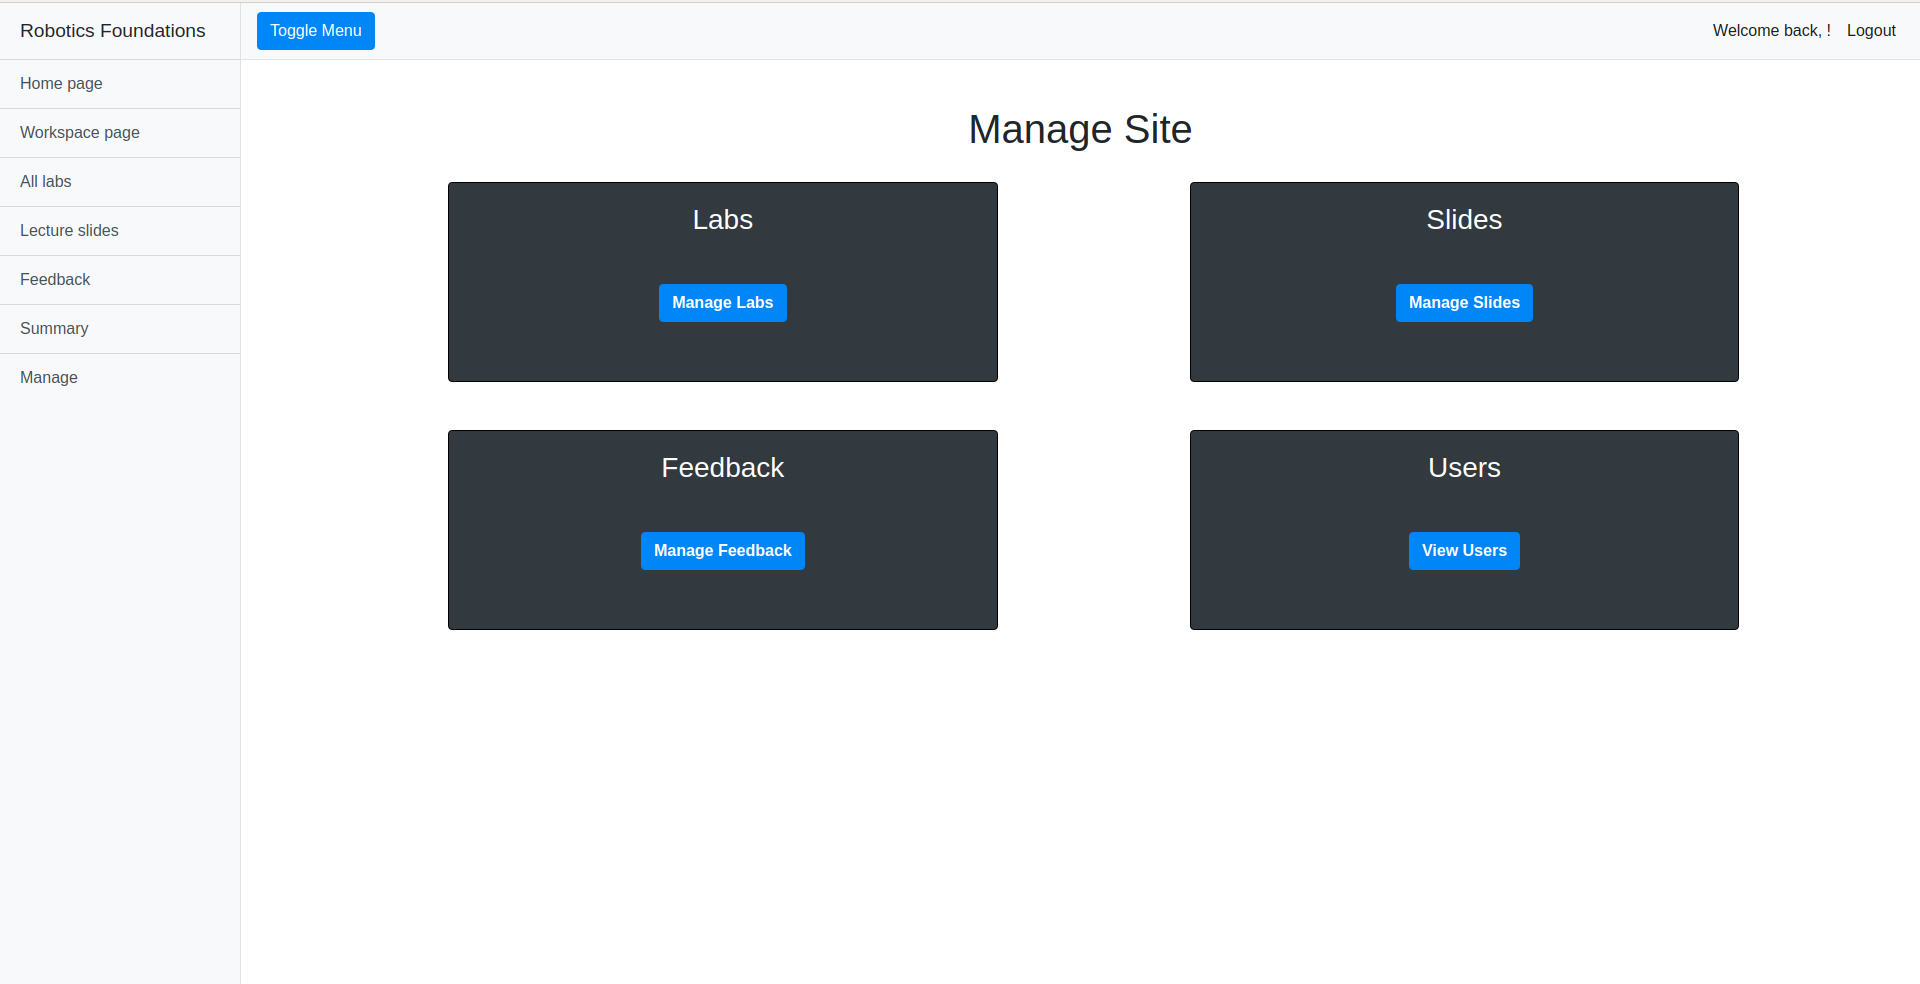
\includegraphics[scale=0.2]{images/admin_manage.png}
    \caption{RFWA's admin management page.}
    \label{fig:manage_page}
\end{figure}

\subsection{Home Page (Iteration 3)}

A home page was created to host several to-be-implemented features which were outlined in the final iteration. A how-to-use guide was displayed here to introduce the web application to new users and demonstrate some of its features to ensure that students can use them properly. A calendar which displayed upcoming due dates were displayed here. Given that users will be redirected to the homepage after a successful login, it made sense to implement the incomplete lab alerts here. Below shows the RFWA homepage with an incomplete lab reminder. The implementation of these features will be discussed in the next section.

\begin{figure}[h]
    \centering
    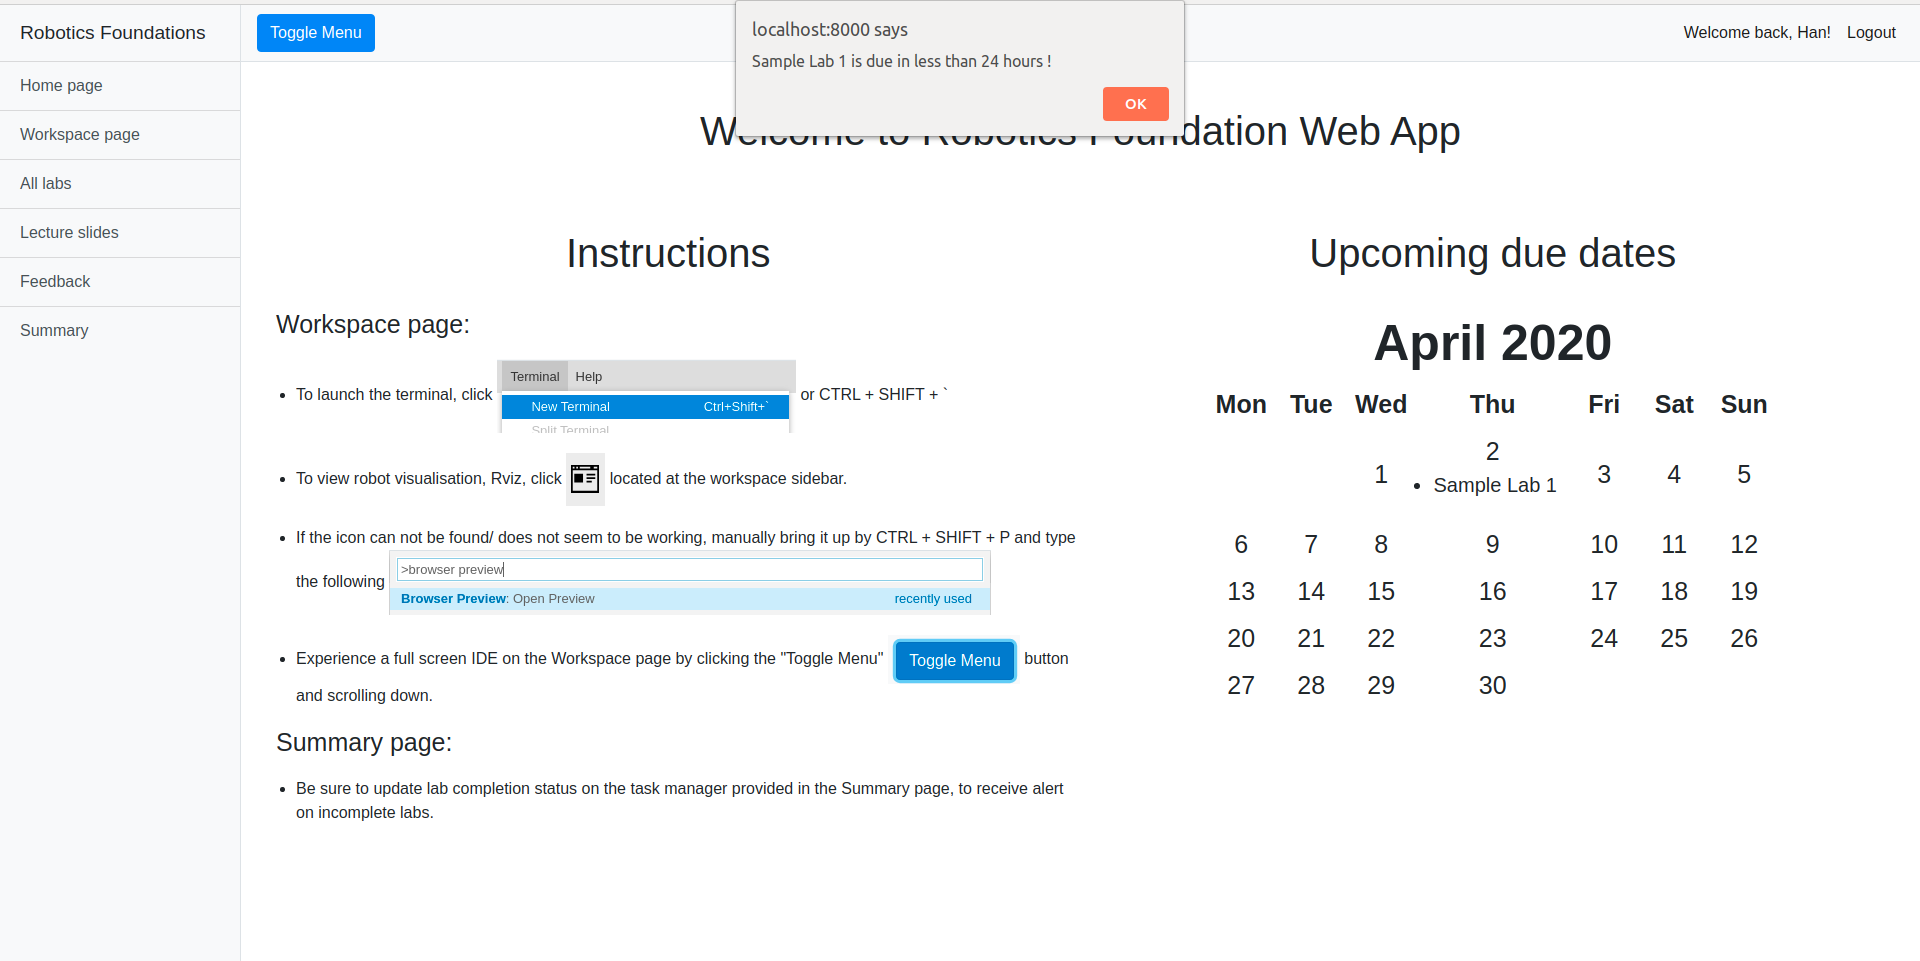
\includegraphics[scale=0.2]{images/home_page.png}
    \caption{RFWA's Home page with an incomplete lab reminder.}
    \label{fig:home_page}
\end{figure}

\subsection{Lab Submission Page (Iteration 1)}

As this project aimed to be a centralised application, not only it should allow users to complete their labs, but also provide features which support the entire lifecycle of a lab exercise. Therefore RFWA should facilitate the handout, completion and submission of a lab exercise. At present, students submit completed labs through submission links provided in the RF course Moodle page. However, RFWA was unable to obtain the Moodle's submission API due to availability and permission issues. Therefore, the submission feature had to be omitted in the final product.

\section {Technology Changes}
Multiple technologies were considered but ultimately dropped in the final product. These included tool limitations and discovering an easier method to implement core features. This section intends to provide insight into how these technologies solve the problem at hand and why they were ultimately replaced. 

\subsection {JupyterLab (Iteration 1)}

Being in the Project Jupyter family, JupyterLab came with Jupyter notebook support but it lacks the ability to view ROS visualisation. This can be solved by implementing the \cite{rosjupyter} widgets or linking external services. The widgets are plugins to the Jupyter ecosystem designed to make working on ROS inside JupyterLab easier. The ROS3D Jupyter widget allows user to view robot visualisations in JupyterLab. However, this widget is developed upon the \cite{rwt} by \cite{rwtpaper}. The project supervisor stated that he did not want tools from Robot Web Tools as they are not featured-packed and contained bugs. Therefore, linking external services was needed to provide ROS visualisation.

Eclipse Theia is a modular IDE framework that allows for customisation, which makes it easier to link external services. Unlike JupyterLab, Eclipse Theia's basic browser application does not provide Jupyter notebook support. Both JupyterLab and Eclipse Theia provides excellent terminal support. This solves the \cite{Butterfly} reliability issue which plagued the previous L4 project. Many factors were considered when deciding between JupyterLab and Eclipse Theia. These included community support and adopters. JupyterLab provided better community support in multiple forums and have a higher number of adopters. There is only 1 active community support forum for Eclipse Theia and less number of users. This is because the targeted end-users for these online IDEs are different. JupyterLab's end users can range from a python beginner to an experienced data scientist. While Eclipse Theia focused on providing the necessary tools for a developer intending to build an online IDE to meet end-user requirements. In the end, it was agreed upon that Eclipse Theia would be used on the workspace page, as it was believed to be the most appropriate tool for this scenario.

\subsection {JupyterHub (Iteration 2)}

Implementing Jupyter Notebook was a priority in the second iteration as it provided IPython kernel support. This is further discussed in later chapters.  Without Jupyter Notebook, users will not be able to complete lab exercises as they are unable to code. Launching a local Jupyter Notebook server provided a web link which can be accessed from a web browser. To produce a clean workspace area, the Jupyter Notebook should be ideally displayed on the workspace page. Therefore, it had to be accessed through Eclipse Theia's inbuilt web browser. Due to security permissions in both Eclipse Theia's browser and Jupyter Notebook, the inbuilt web browser is not able to access the link generated by Jupyter Notebook's server. 

\cite{JupyterHub} can offer notebook servers to a class of students, a corporate data science workgroup, a scientific research project, or a high-performance computing group. It spawns, manages, and proxies multiple instances of the single-user Jupyter notebook server. This ensures that all security requirements in both Eclipse Theia and Jupyter notebook were met. Ultimately, the python package for Visual Studio was imported as an Eclipse Theia plugin, this was a quicker and easier alternative which provided Jupyter Notebook support.

\subsection {Third-Party Django Packages (Iteration 3)}

There are a wide variety of third-party Django packages which users can choose from. 
The benefits of a Django package include saving time and cutting down on boilerplate code by implementing ready-made abstract tools developed by members of the Django community.

In this case, several Django calendar packages were researched for the displaying upcoming due labs in the home pages. These Django packages were extremely easy to implement, however, several were no longer actively maintained and unsupported by newer versions of Django. Some newer packages had poor documentation which made implementation challenging while other packages were providing unnecessary complex features such as rearranging items in the calendar dates. Ultimately, a calendar class was defined in "utils.py" and querying was done in Django's view to render the calendar with upcoming due dates to the user in RFWA's homepage. 

%==================================================================================================================================
\chapter{Implementation}
This chapter will review the implementation stage of the system. First, software engineering
tools that were used will be examined. A progress update is provided for each iteration, followed by an introduction to the technologies used in the final product. Finally, an in-depth 
explanation for the implementation of the system's features will be provided.

\section{Software Engineering Tools}
Given the scale of the project several, software engineering tools were used to provide better life cycle management. These tools do not impose strict schedules and roles, but merely make it easier to self-manage and converge on development goals. 

\subsection{Project Management}

A \cite{Trello} board was used throughout RFWA's development. This enabled easier management of issue tracking and made it possible to find out what was completed and needs to be done. These features were sorted by priorities outlined by supervisor (features that needed to be implemented before the next meeting) and the MoSCoW method mentioned in requirements gathering.  

\begin{figure}[h]
    \centering
    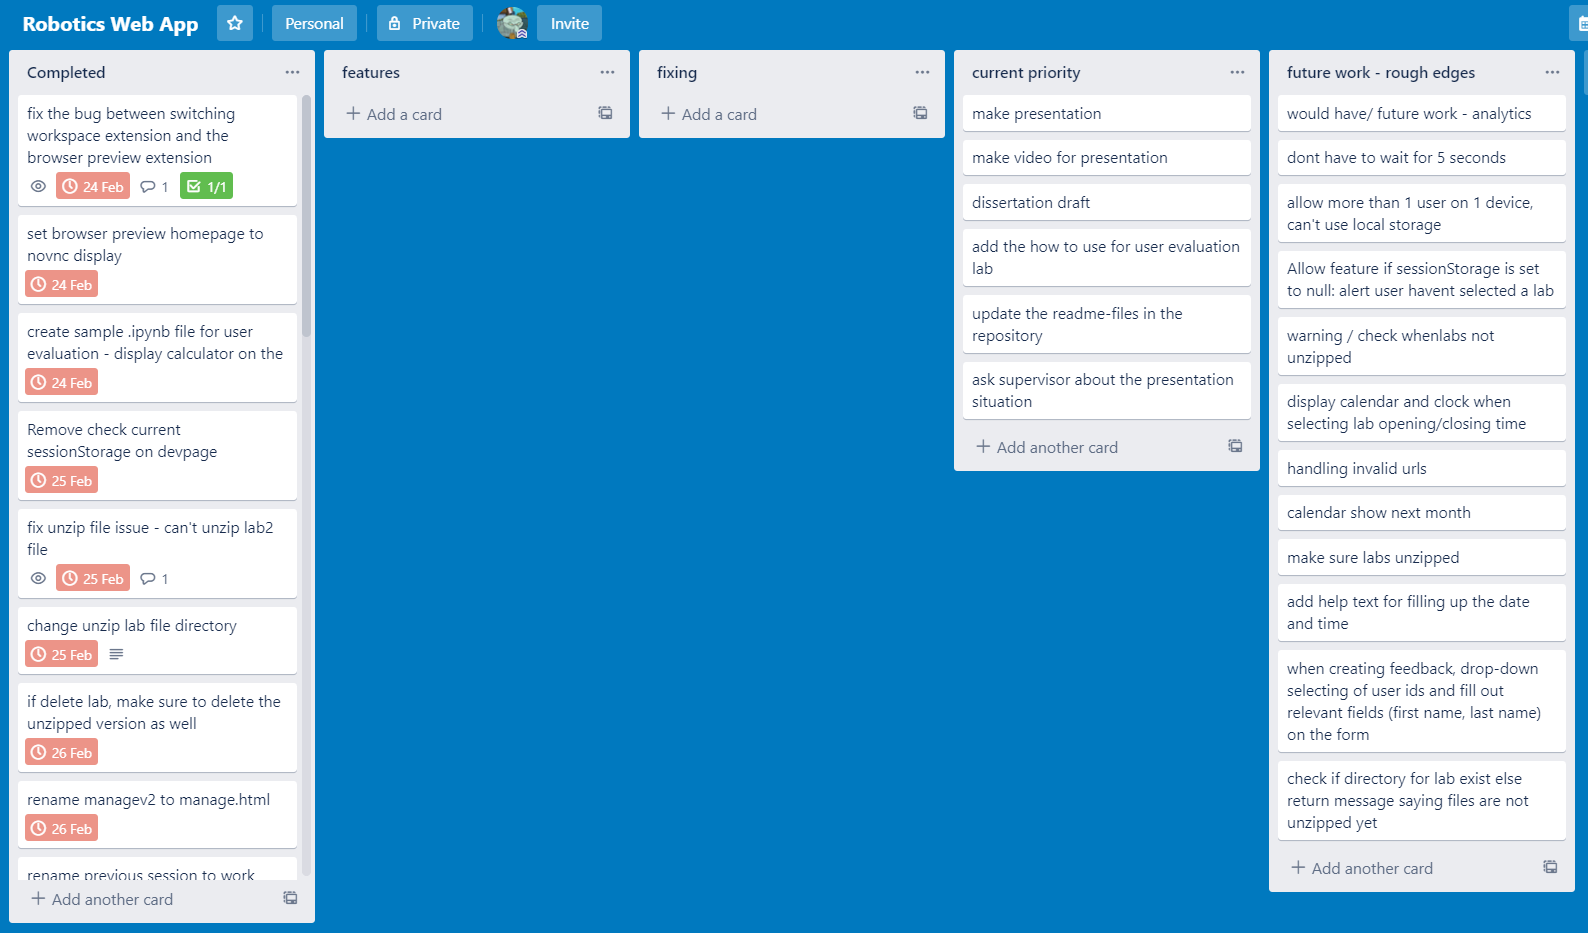
\includegraphics[scale=0.33]{images/trello.png}
    \caption{Status of Trello board before dissertation writing}
    \label{fig:trello_board}
\end{figure}

\subsection{Version Control}

Version control is a vital software development tool. The project repository ensured that all code was backed up and not been lost had any development issues occurred including laptop theft or broken source code. It allows for accurate tracking of file changes in the project by providing a detailed backlog of file changes. Branching features in version control allowed the implementation of new project features without breaking the existing working product. \cite{Github} was the choice of version control given its popularity and experience using it. 

\subsection{Time Tracking}
A time log was used for time tracking. Time tracking provided insight into the time spent on the project. Furthermore, this granted the ability to estimate the time needed to implement new features based on the time taken to complete similar implemented features. The time log is included in the project repository and updated frequently to ensure it is up to date with the project development.

\section{Iterative Development}

This project adopted an iterative development approach, the entire project was split into 3 main iterations. While there were no exact dates set for each iteration, an estimated time frame and goals were identified. 

\section{Iteration 1}

The primary aim of the first iteration was to develop a core product even if that implied that some functionalities were still missing. This was done through the implementation of RFWA's core features outline in the requirements section. 

The duration of the first iteration was the longest, spanning from the start of the first semester until the beginning weeks of the second semester. This was because extensive background research on requirements and tools was conducted before the start of the development. By the end of this iteration, a somewhat working product was developed without IPython kernel support and the development progress is as follows:

\subsection{Successfully Implemented}

\begin{itemize}
    \item 
    Registration, Login page - Users can create an account to access RFWA features.
    \item 
    Lecture slides page - Users can select and view all upload lecture slides.
    \item 
    Lab page - Users can view all uploaded lab exercise details.
    \item 
    Workspace page - Users can code and view robot visualisation through the implementation of Theia IDE, TigerVNC and noVNC.
    \item
    Manage page - RFWA admin can upload and delete lecture slide and lab exercises.
\end{itemize}


\subsection{To Be Implemented}

\begin{itemize}
    \item 
     Workspace page - IPython kernel support.
\end{itemize}

\section{Iteration 2}

RFWA demonstration to the project supervisor yielded constructive feedback from which a new set of requirements were then generated. The main aim of this iteration was to further reduce the cognitive load of users setting up online workspaces. The newly outlined requirements had to be implemented before conducting user evaluation.

This iteration took about 2-3 weeks as most usability improvements were achieved by modifying existing features. By the end of this iteration, a fully working product was successfully developed and the development progress is summarised below:


\subsection{Successfully Implemented}

\begin{itemize}
    \item
    Lab page - Users can select and switch lab workspaces through a click of a button.
    \item 
    Workspace page - IPython kernel support.
    \item 
    Feedback page - Users can view received feedback.
    \item
    Manage page - Admin can provide feedback to users.
\end{itemize}

\section{Iteration 3}

In this iteration, the project supervisor suggested implementing 3 would-like-to-see features obtained from the user evaluation response. After discussion, it was agreed that functional features such as downloading code and reminders should be developed. The justifications of feature implementations are provided in greater detail in the next chapter. The main aim of this iteration was to implement the 3 outlined features and apply usability improvements where necessary. 

As this was the last iteration, it lasted until the end of the second semester, about 6 weeks. By the end of this iteration, RFWA successfully implemented 4 new features and the development progress is highlighted below:

\subsection{Successfully Implemented}


\begin{itemize}
    \item
    Home page - Users will receive a reminder for incomplete labs due in 24 hours and a calendar to view all upcoming lab due dates.
    \item
    Lab page - Users can download their lab progress.
    \item
    Summary page - Users can update their lab progress in the task manager provided.
    \item 
    Manage page - Admins can view and update feedback provided and improvements to the upload form layout.
\end{itemize}

\section{Languages, Frameworks and Tools}

Given the scale of the project, several technologies were implemented into RFWA to meet its requirements. This section intends to introduce the technologies used in the final product alongside how and why it was used in the context of the project. 

\subsection{HyperText Markup Language (HTML)}
HTML is the backbone of any web application, it structures documents to be displayed in a web browser. It can be assisted by technologies such as Cascading Style Sheets and scripting languages such as JavaScript. HTML is used to display contents on RFWA ranging from lab exercise details to calendar displaying upcoming due dates. 

\subsection{Cascading Style Sheets (CSS)}
CSS is a style sheet language used for describing the presentation of a document written in HTML. CSS is used in RFWA to achieve consistency by having the same button colours and providing a pleasant user interface by ensuring sufficient spacing between contents in RFWA.

\subsection{JavaScript}
JavaScript is a scripting or programming language that allows the implementation of complex features on web pages. JavaScript is used to implement features such as menu bar toggling and displaying event messages. Event messages are used for communication from RFWA to the user.

\subsection{TypeScript}
TypeScript is a superset of JavaScript which provides optional static typing, classes and interfaces. This allows for better code structuring in larger-scale projects. In this project, TypeScript is used to create custom extensions in Eclipse Theia.

\subsection{Python 3}
Python3 is a programming language that is required by the Django framework. While Django supports Python 2 and 3, it is recommended to use the latest version of Python 3. Newer versions of Django, supported by Python3, provided better security and more features. Python modules are also used to implement some of RFWA's features such as downloading labs and incomplete lab reminders.

\subsection{Bootstrap}

\cite{Bootstrap} is a CSS framework directed at responsive, mobile-first front-end web development. It contains CSS- and JavaScript-based design templates for typography, forms, buttons, navigation, and other interface components. This project implemented a bootstrap theme which was sourced from a third-party library. There are numerous benefits of bootstrap implementation. First, there are countless websites which provide a wide selection of pre-built templates that ensures consistency. It can be deployed quickly by downloading and adding the bootstrap class name to the HTML elements. Lastly, creating a responsive and pleasant design can be time-consuming. This freed up more time to be spent on developing the core features of RFWA instead of deciding on an insignificant presentation detail. 

\subsection{JQuery}

\cite{jQuery} is a JavaScript library which simplifies HTML document traversal and manipulation, event handling, animation, and Ajax. jQuery is required in the implementation of certain RFWA features such as switching lab workspaces (event handling) and bootstrap navigation bar toggling (CSS animation).

\subsection{Eclipse Theia}

\cite{EclipseTheia} is an IDE framework for desktop and web applications. It is implemented in TypeScript and emphasises extensibility. Eclipse Theia supports deploying as a browser and electron application. Given that RFWA is a web application. It was only logical to deploy Eclipse Theia as a web browser application.

Eclipse Theia was the framework of choice as it offers a wide variety of tools and a high degree of customisation. Eclipse Theia's modular design allowed for specifying required node.js packages in the package.json file. For example, "@theia/terminal" is needed in the package.json file which allows for terminal access when the browser application is rendered. It provides better understanding on the workflow of the project as all dependencies are listed here. Furthermore, Eclipse Theia is based on Visual Studio Code (VS Code), a highly popular and powerful desktop IDE. It reuses components which are used in VS code, such as \cite{xtermjs} for terminal support and \cite{monacoeditor} for code editing. It also came with VS Code's colour theme which provided support for dark theme. This was a requested feature in the previous L4 project. By reusing the same components, it provides a sense of familiarity for VS code users when using RFWA's workspace.

\cite{VSMarketplace} let users add languages, debuggers, and tools to support and improve development workflow in VS Code. Eclipse Theia allows VS Code extensions to be integrated within it, they are imported into Eclipse Theia as plugins. This is further explained in Jupyter Notebook support. Users unsatisfied with the plugin choices can develop their own Eclipse Theia extensions to meet their needs. The main difference between an Eclipse Theia extension and plugin is that plugins can be installed at runtime and they do not affect the stability of the base tool. 

\begin{figure}[h]
    \centering
    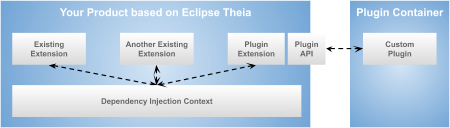
\includegraphics[scale=0.75]{images/extension_plugin.png}
    \caption{Representation of Eclipse Theia's extensions and plugins system.}
\end{figure}


In short, Eclipse Theia is the framework used in RFWA's workspace page as it is the only framework in allowing the creation of a completely custom IDE.

\subsection{Django}
As mentioned above, \cite{Django} was the web framework of choice for the web application. This was for several reasons including previous experience with the framework, project supervisor's experience and Django touted itself as a "batteries included" framework. Being a "batteries included" framework, Django came with a login view, database connection (SQLite), URL handling and more. Given that most of the important components are picked, project development can start right away rather than figuring out things such as authentication, templating engine and database connection.

Django's templating engine allowed HTML code to be shared among multiple page without the need for rewriting code. This is achieved by creating a base template 'base.html'. The bootstrap navigation templates are coded in 'base.html' so that it can be reused in other pages. This provided a similar layout structure across different pages in the Django web application while saving time and minimising recoding errors. Content pages such as 'lectureslides.html' and 'feedback.html' extends from the base template and only additional contents are coded here. Django's URL handling allowed for object querying. For example, the admin uploaded an incorrect lecture slide and wants to delete it. URL handling allowed us to provide querying parameters, lecture slide name, to Django's views. The view matches the lecture slide objects based on the name and deletes it. 

\begin{lstlisting}[language=HTML, caption={The slug, typically used in URL for a short label of something, is being passed to Django's URL handling.}, label=lst:slide_deletion_template_to_url]
<a class="btn-link text-white badge badge-danger badge-pill ml-1"
        href="">Delete</a>
\end{lstlisting}

\begin{lstlisting}[language=python, caption={Django's URL handling receives it and sends it to the corresponding view.}, label=lst:slide_deletion_url_to_view]
path("delete_feedback/<slug:slugName>/", views.delete_feedback, name='delete_feedback'),
\end{lstlisting}


Django's template tags allowed for object rendering. For example, feedbacks are assigned to specific usernames and a user wants to check his feedback, if any. Template tags allows us to check if there is any feedback assigned to the user. If there is, feedback contents would be displayed in the HTML body, else, the user would be notified "You have no feedbacks". This allows for effective communication between the web application and user. Also, this prevents the user from staring at a blank screen, thinking that the web application is loading slowly. 

\begin{lstlisting}[language=HTML, caption={Django's template tag is used to check and display user feedback.}, label=lst:feedback_page]
 <!-- Feedback -->
  
  <div class="table-group">
    <div class="title-group">
      <h1 class="col-12 text-left table-header">Feedback
      </h1>
    </div>

    <table class="table table-hover">
      <thead>
        <tr>
          <th scope="col">Week</th>
          <th scope="col">Grade</th>
          <th scope="col">Comments</th>
        </tr>
      </thead>
      
      <tbody>
        <tr>
          <td>{{feedback.week_number}}</td>
          <td>{{feedback.grade}}</td>
          <td>{{feedback.comments}}</td>
        </tr>
      </tbody>

      
      
      <h2 class="text-center mt-5">You have no feedbacks.</h2>
    </table>
    
  </div>
\end{lstlisting}

\subsection{TigerVNC and noVNC}

\cite{TigerVNC} and \cite{noVNC} are the VNC tools which were used in the previous L4 project. Given that the project supervisor did not had any complaints about it, it was decided that the same VNCs would be reused again, adhering to the "if it’s not broke don’t fix it" principle.

TigerVNC is a high-performance, platform-neutral implementation of VNC that allows users to launch and interact with graphical applications on remote machines. TigerVNC provides the levels of performance necessary to run 3D and video applications, and it attempts to maintain a common look and feel and re-use components, where possible, across the various platforms that it supports. On the other hand, noVNC is both an HTML VNC client JavaScript library and an application built on top of that library that runs well in any modern browser. In the context of this project, TigerVNC is used to create a virtual display and noVNC forwards the display by generating an accessible link to it.

\section{Registration and Login Page}

This is the page where user registration and login takes place. New users begin the registration process by filling out the required details such as username, first name, last name, password and password confirmation. Django's built-in user registration system included several validators to prevent the use of weak passwords. User passwords can not be too basic (cat123), entirely numerical or similar to user's username, first name and last name. A royalty-free image was added into the background of these pages. 

Users have to enter their login details, username and password. Users will be redirected to the home page after a successful login. This is done by specifying the LOGIN\textunderscore REDIRECT\textunderscore URL in Django's settings. All users must be logged in to access RFWA features and are enforced using 'user.is\textunderscore authenticated' tag in base.html and '@login\textunderscore required' decorator in views.py,


\begin{figure}[h]
    \centering
    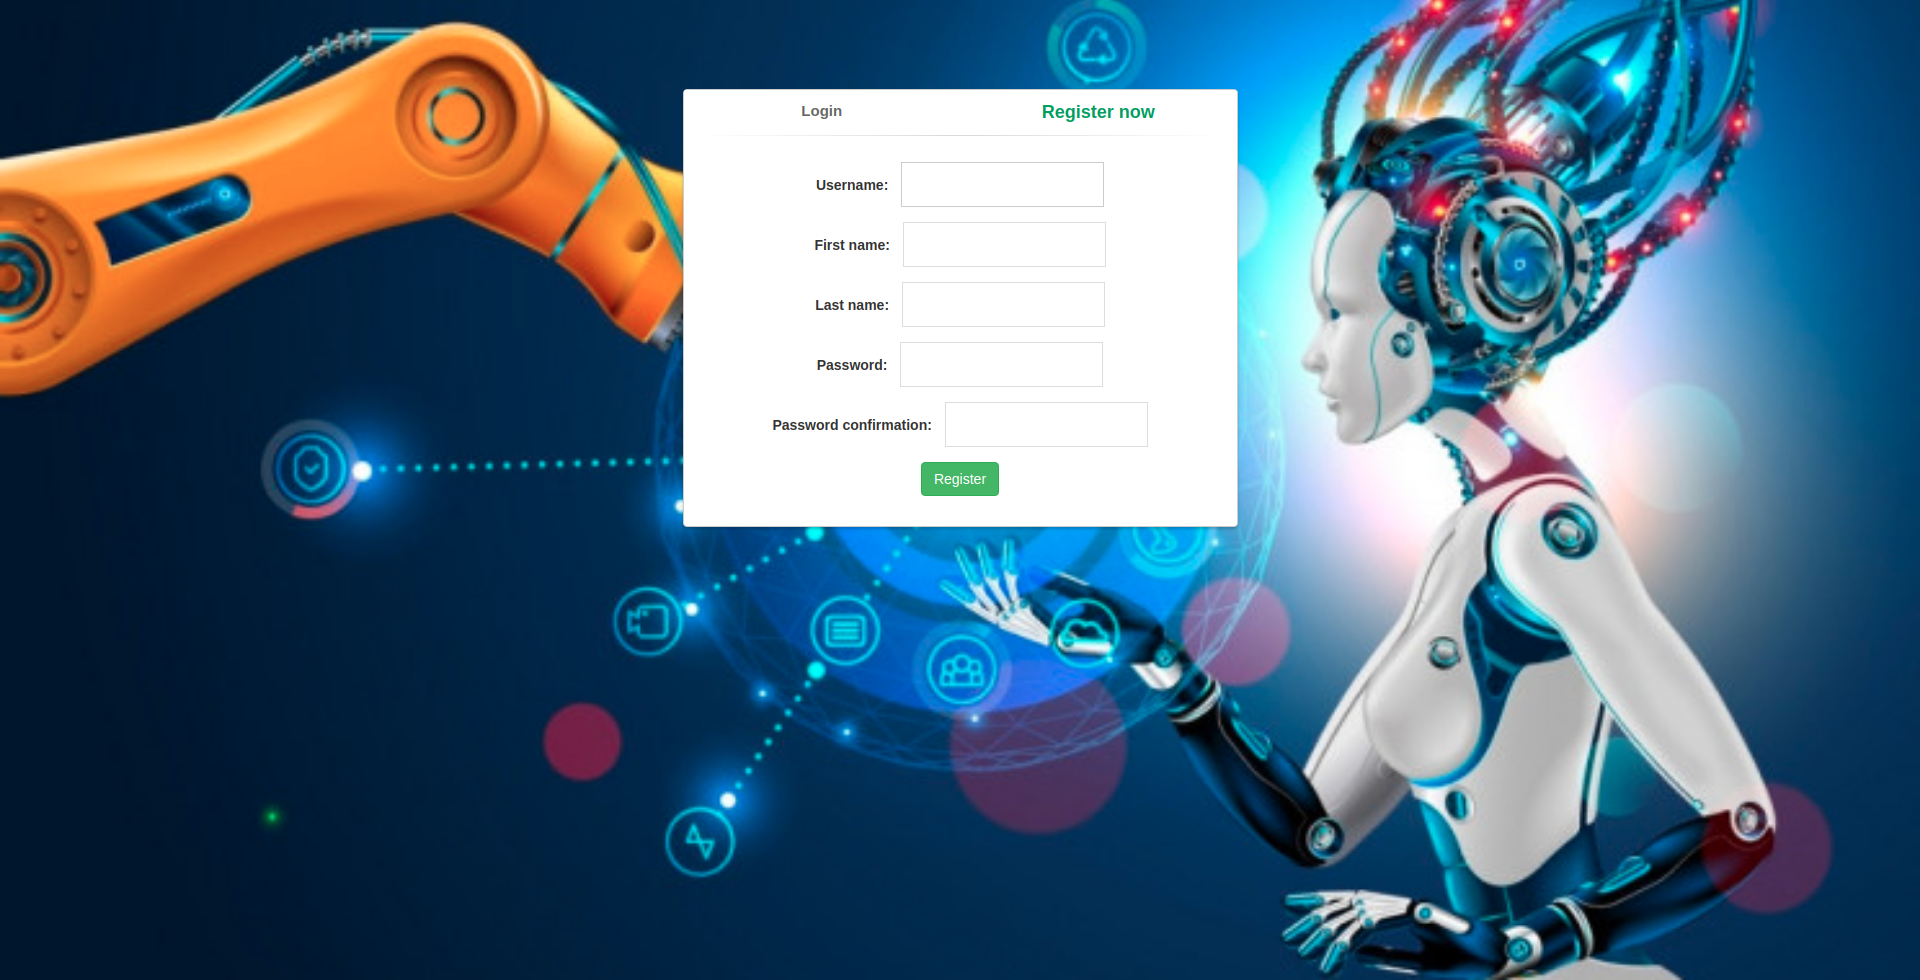
\includegraphics[scale=0.2]{images/registration_page.png}
    \caption{Registration Page.}
    \label{fig:registration_page}
\end{figure}


\subsection{Username Sanitation}
RFWA admins provide feedback to individual users by assigning them based on usernames. It would be less confusing and much simpler to provide feedback to a username which is a student ID, 2288527l compared to haggislover22. Therefore the registration page only accepts user's student id as the username. This was implemented by extending the Django's default user creation form and adding a sanitising input method. Since all student ID have the same format, 7 digits followed by 1 letter, the sanitising method checks if the username format is met before proceeding with user creation. Help and warning texts can be further customised for different requirements. In this scenario, warning text "Must be student ID" is displayed when the username does not meet the formatting requirements.

\begin{lstlisting}[language=python, caption={Sanitising username performed in forms.py.}, label=lst:username_sanitising]

def clean_username(self):
        data = self.cleaned_data['username']

        # 3 checks, check length = 8, the last letter must be an alphabet, the first 7 must be numbers
        if len(data) == 8 and data[-1].isalpha() and data[:-1].isdecimal():
            return data
        else:
            raise forms.ValidationError("Must be student ID")
\end{lstlisting}

\section{Home Page (Iteration 1)}

The home page of the application, shown in Figure \ref{fig:home_page}, is where the user is redirected to after a successful login. As mentioned in previous sections, several features are implemented here. These are user onboarding, incomplete lab reminder and a calendar displaying labs due in the current month. The implementation of these features is described below.

\subsection{User Onboarding (Iteration 3)}

A mini user guide is included on the left half on the home page. It was necessary to create a user guide so that new users can acquire the necessary skills to become effective users of RFWA. With new users being able to make the most out of RFWA, this meant that there will be less environment set up issues for admins to look into. 

\subsection{Reminder (Iteration 3)}

This requested feature was implemented in the third iteration after conducting user evaluation. Users will be reminded if there is an incomplete lab due in 24 hours. The task manager in Summary page allows users to update their lab completion progress by ticking checkboxes. Project supervisor also specified that users should only be reminded once on the home page each time they log in.  

Django's home page view queries a list of labs which are due in less than 24 hours and passes it to 'homepage.html' in JSON format. Completed labs names are stored in the web browser's localStorage. The web application compares and checks if the lab names returned from Django's view exist in the web browser's localStorage. If user has not complete the lab and warned, JavaScript is used to create an alert. Users will have to acknowledge the alert by closing it before being able to navigate to other pages in RFWA. 

Once a user is reminded, it changes the key value ("warned") to True in the web browser's sessionStorage. Therefore, the users will not be warned twice on subsequent home page visit in the same browsing session. localStorage and sessionStorage both allows for data storage in the web browser, but with sessionStorage the data is persisted only until the window or tab is closed, while with localStorage the data is persisted until the user manually clears the browser cache or web application clears the data.

\begin{lstlisting}[language=HTML, caption={JavaScript code implementation of the incomplete lab reminder feature}, label=lst:reminder]
<script>
  window.addEventListener('load', function () {
    var received_data = jQuery.parseJSON('{{name_json | safe}}');
    var due_labs = [].concat.apply([], received_data);

    // check if user has been warned before
    if (sessionStorage.getItem("warned") != "true") {
        for (var i = 0, len = due_labs.length; i < len; ++i) {
        if (!localStorage.hasOwnProperty(due_labs[i])) {
        
          // display alert
          alert(due_labs[i] + " is due in less than 24 hours !")
          
          // set warned status to true
          sessionStorage.setItem("warned", "true")
        } else {
          console.log("you have completed " + due_labs[i])
        }
      }
    }
    console.log(sessionStorage)
  })
</script>
\end{lstlisting}

\subsection{Calendar Display (Iteration 3)}

Similar to the reminder feature, this feature is implemented during the third iteration. A new python class, Dateline Calendar, was extended from python's default HTML calendar. Dateline Calendar generated a basic HTML calendar based on current month and year values with the name of  due labs. Django's view then passes the HTML calendar to 'homepage.html' and rendered as a HTML code, displaying the calendar with upcoming due dates.

\section{Workspace Page (Iteration 1)}

Users will conduct their lab exercises in the workspace page, shown in Figure \ref{fig:workspace_page}. This page can be accessible either by directly clicking the 'Workspace Page' on the navigation sidebar or by selecting a lab in 'Lab Page'. Directly clicking 'Workspace Page' will resume the saved workspace where the user left off in the previous session. 

Eclipse Theia is embedded in the workspace page via iFrames. The iframe attribute 'src' specifies the address of the document to embed in the <iframe> tag. Address of Eclipse Theia's browser application can be obtained by the terminal command 'yarn run start'. Users can code and visualise robot simulations with the implementation of the following features described below. 


\subsection{Jupyter Notebook Support (Iteration 2)}

Jupyter Notebook support was implemented through an Eclipse Theia plugin. The \cite{pythonextension} supported coding in Jupyter Notebook alongside other features such as IntelliSense and code formatting. IntelliSense made coding editing easier with auto-completion, code navigation, syntax checking. The python extension was downloaded from the Visual Studio Code marketplace. A new folder named 'plugins' had to be created inside Eclipse Theia's project directory and all downloaded VS Code extension files (.vsix) will be placed in here. This specified a directory to be scanned for plugins. All plugins contained in this directory will be added automatically when Eclipse Theia is launched. To enable the extensibility via plugins in general, the “@theia/plugin-ext” extension has to be included in Eclipse Theia's package.json file.

The VS Code python plugins successfully provided Jupyter notebook support. However, there are some minor issues with it. In \cite{theia0.15.0}, the python plugin is only activated upon editing a python (.py) file. This resulted in Jupyter notebooks being rendered in an unwanted way and prevented users from coding. This meant a python file (test.py) had to be included in the sample labs that was used in during user evaluation. This issue was fixed in \cite{theia0.16.0}, which was rolled out at the end of February. 

\subsection{Viewing Robot Visualisation (Iteration 1)}

This feature was implemented using VNCs mentioned above and importing the \cite{browserpreview}. On the server-side, ROS, Gazebo, TigerVNC and noVNC would be installed in a supported environment. TigerVNC would be used to create a virtual display and noVNC generates a forwarding link to access it on a web browser. Gazebo and Rviz are exported to the virtual display. The client-side (Eclipse Theia in RFWA's workspace page) can access the virtual display through the forwarding link from noVNC.

To make it as easy as possible to access these features, minimal user typing and clicks are enforced here. By specifying a port forwarding number, noVNC can generate a constant, unchanged forwarding link which is used to set the home page of a web browser in Eclipse Theia. However, the Eclipse Theia's in-built web browser does not support user preference which meant that its browser home page could not be set. To fix this, the Browser Preview extension for VS Code was implemented as an Eclipse Theia plugin. This provided the ability to set the default startUrl (noVNC port forwarding link) and have multiple browser previews open at the same time.

\section{Lab Page (Iteration 1)}

In this page, users can view all uploaded labs sorted by its due date. Relevant lab details such as lab name, description and due date are displayed here. Users can choose the lab to work on by clicking on the blue load lab button and download their lab progress through the red download button. The implementation of both these features is described below. 

\subsection{Switching Workspace (Iteration 2)}

Eclipse Theia loads the last workspace in the previous session on start if the current session does not specify a workspace directory. For example, Tim was working on Lab Week 2 on his last RFWA session yesterday. Today, he wants to work on Lab Week 3 but the workspace for Lab Week 2 is loaded instead. Tim can manually change the workspace using "File" -> "Open Workspace". However, this method is not user-friendly and users might open the wrong workspace directory. With the project aim (reducing user cognitive load during lab set up) in mind, a feature had to be implemented. This feature was implemented via an Eclipse Theia extension. 

Given a workspace directory, the frontend API 'workspaceService.open' opens the provided workspace directory in the same window. RFWA has to pass this workspace directory to Eclipse Theia's extension. A postMessage implementation is required for cross-domain communication. When a user clicks on the 'Load Lab' button, a postMessage() method sends the new workspace directory, a file URI, to Eclipse Theia. However, Eclipse Theia has to be rendered on the iframe before receiving the file URI to enable a workspace switch. Therefore, 5 seconds of waiting time is needed to ensure that Eclipse Theia is always present on the iframe before the web page calls the postMessage() method. When Eclipse Theia's extension receives a workspace directory to be opened, it will ask if the user has any unsaved progress. If yes, the page reload will be suppressed and the user can proceed to save. If there are no unsaved progress, Eclipse Theia is reloaded in the new workspace.

\begin{figure}[h]
    \centering
    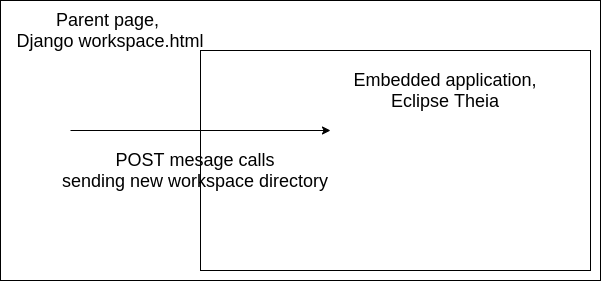
\includegraphics[scale=0.65]{images/postMessage_diagram.png}
    \caption{Sending of a new workspace directory through postMessage().}
    \label{fig:postMessage_implementation}
\end{figure}

\subsection{Downloading Labs (Iteration 3)}

Users may want to download labs for several reasons such as backup or future references. A new Django view was used to implement this feature. The view begins by zipping the user's workspace. The zipped file is named by the following format 'username\textunderscore lab name' for easier identification. An HTTP response is generated and it begins the file download. Once this is done, it deletes the user's zipped file so that it can provide more free space in RFWA. Multiple python OS functions are used in the Django views to zip and name the files.

\begin{lstlisting}[language=python, caption={Code snippet from Django's download\textunderscore lab view which zips and allow users to download lab files.}, label=lst:download_lab]
 # zipping file
 shutil.make_archive(output_file_name, 'zip', unzipped_lab_path)

 # changing to base directory
 if (os.getcwd() != settings.BASE_DIR):
 os.chdir(settings.BASE_DIR)

 # downloading the zipped file
 filename_with_type = output_file_name + ".zip"

 lab_directory = os.path.join(settings.MEDIA_ROOT, "labs")

 zip_file = open(os.path.join(lab_directory, filename_with_type), 'rb')
 response = HttpResponse(zip_file, content_type='application/force-download')
 response['Content-Disposition'] = 'attachment; filename="%s"' % filename_with_type

 # deleting user's zipped file
 os.chdir('media/labs')
 os.remove(filename_with_type)

\end{lstlisting}

\section{Lecture Slides Page (Iteration 1)}

In this page, users can view uploaded lecture slides. Upon clicking a 'View slide' button, the lecture slide (.pdf) file would be open in a new browser tab. This allowed users to go back to the RFWA tab to open more slides and access other features of the web app, providing better user experience. This was implemented in the 'onclick' attribute in the HTML button tag.


\begin{lstlisting}[language=HTML, caption={Django's template tag is used to check if a user has received any feedback}, label=lst:view_slide]
 <button class="btn btn-primary font-weight-bold" rel="noopener noreferrer"
    onclick="window.open('../../media/{{slide.lecture_Files}}','_blank')">
    View
 </button>
\end{lstlisting}

\section{Feedback Page (Iteration 2)}

In this page, users can view feedback provided by supervisors. This design is fairly basic as all feedback are arranged in an HTML table format. Despite being plain and simple, the table displays all details in a feedback. Code snippets can be found at Listing \ref{lst:feedback_page}


\section{Profile Summary Page (Iteration 1)}

In this page, users can view their account details and update the task manager. The task manager is a feature that was added during the third iteration which synergises well with the lab reminder feature on the home page. 

\subsection{Task manager (Iteration 3)}

The task manager displays all available labs with a checkbox next to it. Users can update their progress by ticking the boxes and saving box status. When the save button is clicked, it clears all values in the local storage, before adding the checkbox IDs which are checked. By implementing 'localStorage.clear()', it deletes any unchecked checkboxes which might be previously checked and stored in the localStorage. Checkboxes are repopulated each time the profile summary is loaded. A javascript event listener waits for the page to load then retrieves the checkbox ID which are checked and proceed to check the boxes.

\begin{lstlisting}[language=HTML, caption={JavaScript code snippets used to save and repopulate checkboxes.}, label=lst:task_manager]
// saving checkbox values to local storage
function save() {
  localStorage.clear();
  var checkboxes = document.getElementsByClassName("lab-name");
  for (checkbox of checkboxes) {
    if (checkbox.checked == true) {
      localStorage.setItem(checkbox.id, checkbox.checked);
    }
  }
}
// repopulating checkboxes
 window.addEventListener('load', function () {
    for (var i = 0, len = localStorage.length; i < len; ++i) {
     if (localStorage.getItem(localStorage.key(i)) == "true") {
      var checkbox_id = localStorage.key(i)
      document.getElementById(checkbox_id).checked = true;
    }
  }
})
\end{lstlisting}


\section{Manage Page (Iteration 1)}

This page is where admins have access to several actions implemented. The actions (uploading, updating, deleting and viewing) are implemented to ensure that contents in RFWA can be properly managed. This page is only visible in the navigation sidebar to RFWA admins. Any standard user attempting to access the manage page by entering the URL 'rfwa/manage/' will be logged out. Showed in Figure \ref{fig:manage_page}, the manage page allows admins to manage labs, slides, feedbacks and view all registered users. Admins can select what content they want to view.

\subsection{View Content (Iteration 2)}

4 separate pages were created to allow admins to view existing contents. Admins can view uploaded labs, slides, feedbacks and all registered users. The uploaded contents are displayed in a basic HTML table format and necessary actions are provided.

\begin{figure}[h]
    \centering
    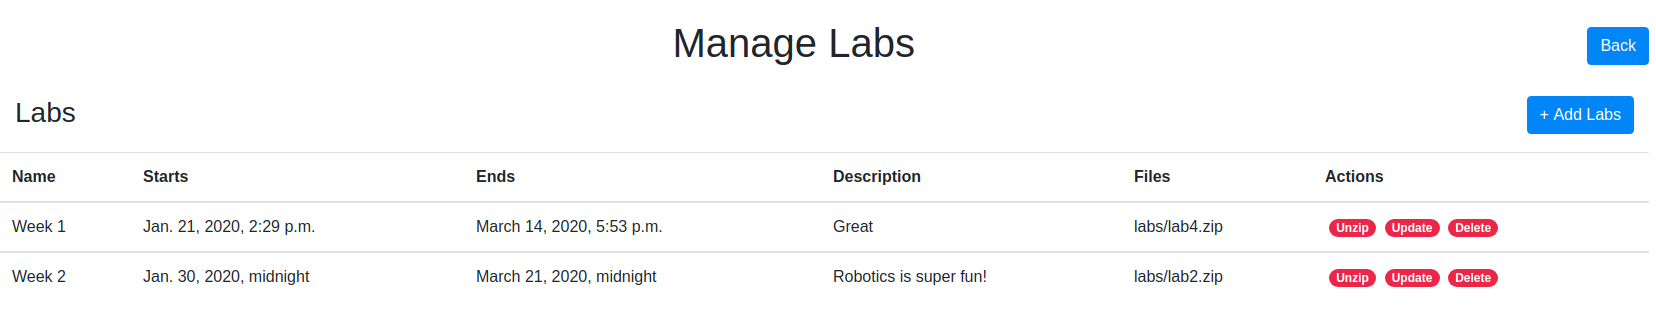
\includegraphics[scale=0.22]{images/manage_labs.png}
    \caption{Manage Lab page after choosing 'manage labs' in the manage page}
    \label{fig:manage_content}
\end{figure}

\subsection{Upload Content (Iteration 1)}

This feature allowed admins to upload labs, slides and feedback. An upload form for these items is defined in Django's forms. These forms have different fields. For example, lab forms have 5 fields (name, description, open date, close date and files) while lecture slide forms have 2 fields (name and files). Some form fields provided a space for users to key values in, while others provided a drop-down selection of all available options to choose from. For example, admins can key in any lab name but only choose from a grade range (A1 to H0) when providing feedbacks. All fields have to be filled to be considered as a valid form. A cancel button is provided if admins decide to not continue the current upload process. They will be redirected back to the management page, shown in Figure\ref{fig:manage_content}. 

\subsection{Unzip Content (Iteration 2)}

Apace page. This feature is only available in lab management as it is not required in the management of other contents. There is no file upload for feedbacks, slide files are in PDF format and there are no management actions when viewing users. Django URL handling and view query the object and python zipfile module is used to unzip it. These files are unzipped to a directory in the Django project.

            
\begin{lstlisting}[language=python, caption={Code snippet from Django's unzip\textunderscore lab view which unzips uploaded zipped files.}, label=lst:unzip_content]
with zipfile.ZipFile(lab.lab_Files.url[1:], 'r') as zip_ref:
    zip_ref.extractall('../django_project/media/labs/')
\end{lstlisting}

\subsection{Update Content (Iteration 2)}

Admins can update existing lab and feedback context. For example, if a closing date was incorrectly specified or there are spelling errors in feedback comments, admins would want to update that. Similar to unzipping content,  Django URL handling and views queries the object. A pre-filled lab form of the queried object allows admins to update necessary files. This was made possible by obtaining the instance of the queried object and its instance is then filled into the form. However, not all fields can be changed. Fields which are primary keys (the lab name for lab and slide object, the assigned username and week number for feedback object) can not be changed. 

\subsection{Delete Content (Iteration 1)}

This feature allowed admins to delete labs, slides and feedback. To delete a lab, admins have to click on the delete button provided. Django URL handling and view query the object and delete it.
The queried object can be deleted using 'object.delete()'. However, this does take account of unzipped labs since they are not included in the Lab object. Therefore, python OS and shutil modules were used to delete the corresponding unzipped lab files, if any.



%==================================================================================================================================
\chapter{Evaluation} 
This chapter will detail how the system was evaluated in multiple ways. The results gathered from user evaluation will be discussed. Finally, the system will be validated against the project requirements to see if they were met.

\section{User Evaluation}

As RFWA is designed to be a learning platform for members in the Robotics Foundation course, user evaluation is necessary to determine how effective the system is in achieving its goals. The evaluation conformed to all requirements in the School of Computing Science ethics checklist.

\subsection{Experiment Methodology}

An experiment was developed for effective evaluation of RFWA. The experiments were designed to evaluate the ease of use of the RFWA and its features. Following the experiment, a questionnaire was also filled in by participants to elicit both quantitative and qualitative feedback. Combining quantitative and qualitative techniques allows for a richer and comprehensive understanding of the evaluation results.

In the experiment, participants will take part in completing 5 tasks. A standard RFWA user would be expected to make these 5 interactions to access and make full use of the web application features. These tasks aimed to evaluate the intuition, ease of navigation and workspace usability of RFWA. Sample lab 1 and 2 are created for the experiment. Here, the sample lab 1 contains a Jupyter notebook file which instructs users to bring up a calculator in the virtual display followed by performing a series of mathematical calculations to display their birthday. These tasks and files can be found in Appendix (LABEL). 

11 participants, who had never seen the system before, volunteered to take part in this experiment.  After completing the 5 assigned tasks, users were asked to fill up a post-evaluation questionnaire. Here they would rate how easy it was to complete individual tasks in the experiment. An introduction script and a debriefing script were used to brief and debrief participants at the start and end of the experiment. The scripts were to provide participants with the project and evaluation aims. They were assured that it was the system, not them, that was being evaluated.


\subsection{Quantitative Data}
The quantitative data gathered from the evaluation were the user's opinion on the ease of use when conducting each of the experiment tasks, on a scale of 1 to 5. 1 being very difficult and 5 being very easy. The scores received for each task were mostly positive, with a score of 4 or 5. The lowest rating received was 3 for 'How easy was it to work on lab 1?'

All participants successfully performed a series of mathematical calculation which resulted in the display of their birth date on the first attempt. This meant that the virtual display was extremely easy to interact and operate. The question "Overall, how easy was the web app to use?" received an average score of 4.4 with 7 out of 11 users found it easy and the remaining 4 users claimed it was very easy. This suggested that the non-functional requirement \#1 was met. The final quantitative question, "Overall, what score would you rate this web app" received an average score of 4.5. This meant that RFWA was well-received among participants.

\begin{figure}[h]
    \centering
    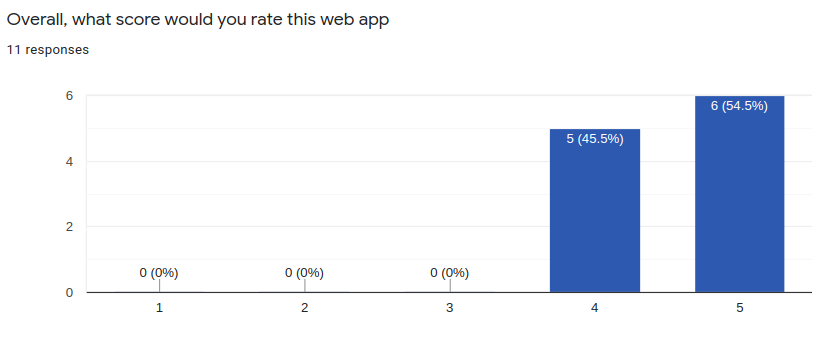
\includegraphics[scale=0.5]{images/overall_results.png}
    \caption{Overall score given to RFWA by participants}
    \label{fig:overall_results}
\end{figure}

\subsection{Qualitative Data}

In terms of qualitative feedback, participants were asked about the features that they liked most, disliked and features to be implemented. This gathered a wide variety of responses. Participants had positive remarks about the UI such as "Easily accessible', "I liked how clean the app looks" and "Layout, the layout is very clear and simple, which easy to use, and the app is working very smooth. Toggle menu feature is very useful." Positive remarks on features were also received. These were "the ability to view your calculator on 1 side and read Jupyter notebook on the other", "the ability to load labs from server" and "I get reminded to save my work before switching".

Only 3 feedbacks on disliked features were received, these suggestion were UI related. They are "The menu could be bigger to make it more readable", "looks boring, maybe a more fun colour scheme" and "The UI is a bit blank, its simple and clear, but could have add more content into it". There was no mention of functional features here, which meant that they were well received among participants. However, one could argue that 15 minutes of user evaluation is not sufficient for participants to identify the functional features that they disliked. A mix of functional and non-functional feature suggestions was received. 2 users did not provide a suggestion due to reasons "can't think of anything" and "no comment - due to lack of personal knowledge". The implementation of suggestions will be further explored in the next section. 

\subsection{Suggested Features from User Evaluation}

As mentioned in previous chapters and section, 3 suggested features will be evaluated and implemented for the third iteration. The following are the suggested features, categorised by its functionality.

The non-functional feature suggestions are:

\begin{itemize}
    \item 
    Make it look more appealing.
    \item 
    More profile customisation to view on my profile page.
\end{itemize}

While the functional feature suggestions are:

\begin{itemize}
    \item 
    Could add a calendar as a reminder for students' upcoming assignments.
    \item 
    A way of downloading the work you've done for submissions.
    \item
    Could have add tutorial about how to use ROS.
    \item
    Can add a search bar to find the keywords that will direct us to the file.
    \item
    A reminder to complete your labs, e.g. 5 hours left and not completed.
    \item
    Link Stack Overflow if a user gets an error message.
    \item
    Hints for the labs in case students get lost.
\end{itemize}

To decide which features were to be implemented, a discussion was held with project supervisor in which it was made clear that to-be implemented features had to be functional. Therefore, features such as 'more profile customisation to view on my profile page' and 'make it look more appealing' were eliminated. It was decided that the top 3 functional features which will add the most value to RFWA should be implemented. Below are the justifications as to why certain features were not chosen and some were to be implemented in the third iteration.

\begin{center}
    Could have add tutorial about how to use ROS.
\end{center}

The addition of this feature would be beneficial to students who are new to ROS. However, this is more of an content addition rather than a new feature implementation. Given that it is an content addition, admins can include ROS tutorials in a separate lab exercise. Furthermore, ROS tutorials might be covered in the RF course and are widely available online. Students can even head to ROSDS, mentioned in the background chapter, which is an excellent ROS learning platform.

\begin{center}
    Can add a search bar to find the keywords that will direct us to the file.
\end{center}

A search bar is a tool that is available on most websites. It allows for quick and easy content retrieval. It is a nice-to-have feature in RFWA, but it adds little to no value at all. This is because there is not much content available for browsing in RFWA. It is not that hard to find and select a file if they are sorted and categorised. This is the case for RFWA, where lab files are sorted by their upload date, lab exercises are separated from lecture slides through different pages and there are 10 files at most to choose from (1 new file uploaded each week for 10 weeks).

\begin{center}
    Link Stack Overflow if a user gets an error message.
\end{center}

The implementation of this feature would boost students productivity when conducting lab exercises. Users debugging process would be resolved quickly. However, like the 2 suggested features above, it adds little to no value to RFWA. Users can just open a new browser tab, navigate to Stack Overflow and search for answers. Furthermore, users might be better off using the previous method if the Stack Overflow linking feature contains bugs. 

\begin{center}
    Hints for the labs in case students get lost.
\end{center}

Similar to "Could have add tutorial about how to use ROS.", this is a content addition. Admins can provide hints in the lab exercise.

\begin{center}
     A way of downloading the work you've done for submissions.
\end{center}

The addition of this feature will allow users to download their lab code. There are a variety of reasons that a user might need this feature, This includes to work on the lab code on their laptop, for storage purposes and revising lab materials for the examinations. This is a useful feature as it adds functionality to RFWA and will be implemented.

\begin{center}
    A reminder to complete your labs, e.g. 5 hours left and not completed.
\end{center}

The addition of this feature would ensure that students complete and submit their lab exercises on time. If a user has an incomplete lab that is due soon, a reminder would pop up and alert the user. Users will have to acknowledge this by clicking "OK" to continue navigating RFWA. This is useful feature which reminds the user of their incomplete labs and will be implemented.

\begin{center}
    Could add a calendar as a reminder for students' upcoming assignments.
\end{center}

The addition of this feature would allow students to view upcoming due dates for the exercises. Students can plan their schedule to ensure that sufficient time is dedicated to lab completion. The calendar would be displayed in a format that students might be familiar with, like the calendar in \cite{SoCS}. This is a useful feature as it allows users to plan and will be implemented.

\begin{figure}[h]
    \centering
    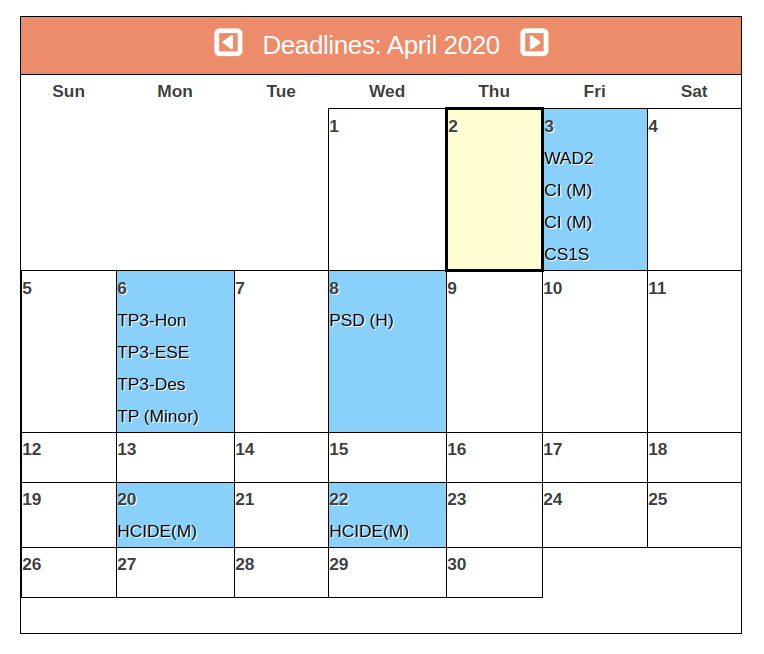
\includegraphics[scale=0.53]{images/calendar-socs.png}
    \caption{Dateline calendar in SoCS online.}
\end{figure}

\section{Unit Testing}

Unit tests were created to ensure the correctness of the code behind the system and that the
RFWA performs as expected. 49 unit tests were created. These unit tests tested various aspects of the application such as URL redirecting, model creation and HTML template rendering. In this project, tests files are split into 3 different files, test\textunderscore forms.py, test\textunderscore views.py and test\textunderscore models.py. This allowed better file management, ensuring that each file only stores the relevant test functions and these files can be executed separately from one another.  

For each page, a set of basic tests were conducted. These included checking if the user is allowed to view a certain page and the proper template loaded. Third-party tools, \cite{Coverage} and Django \cite{Modelmommy} were used as well. Coverage was used to calculate the number of code lines that are executed while the automated tests are running. Django model mommy is used to simplify test model generations by handling all attributes and relations. The overall test coverage averaged 81\% of code coverage. The least code covered file was views.py with 45\%. Most views had error handlings such as "if-else" and "try-except" statements. Furthermore, as views became more complex, so did their testing process. Views that implemented python OS, shutils and zipfile modules were inherently harder to test. It would take too long to generate all test views to meet 100\% test coverage.

\begin{figure}[h]
    \centering
    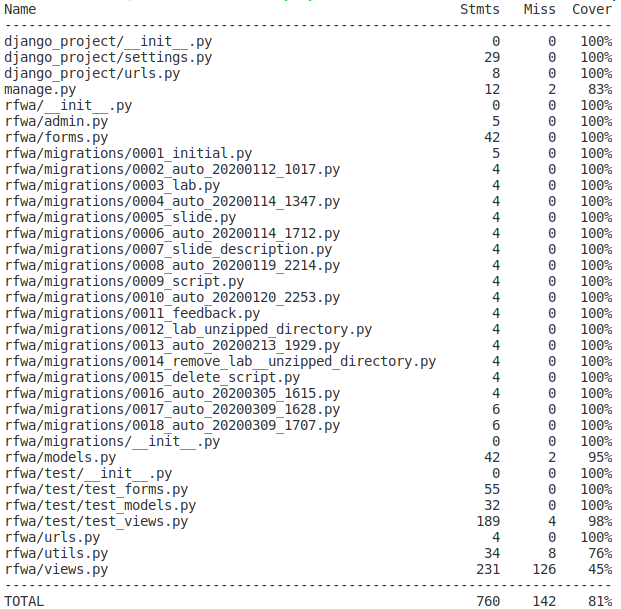
\includegraphics[scale=0.64]{images/coverage_report.png}
    \caption{RFWA test coverage report.}
\end{figure}

\section{Requirements Validation}

The final stage of the evaluation process was to determine if the functional and non-functional
requirements outlined in Section 3 had successfully been met or not. As discussed when these
requirements were stated, several requirements were added throughout the development of the
project, and so only the final set of requirements will be validated. 

Overall, 20 of the 22 Must Have, Should Have and Could Have functional requirements were met by the end of the project - approximately 90\%. All 10 Must Have functional requirements were met; all 6 should have requirements were met; only 2 of the 4 Could Have functional requirements were met. These are "User could be able to customise the theme on the web app" and "Admin could be able to view lab analytics". The requirement "User could be able to customise the theme on the web app" could be considered as partially met as Eclipse Theia provides several inbuilt themes. However, these themes only apply to the workspace page. Due to time constraints in the project, these 2 requirements not met. However, they would provide extra value to RFWA and should be included in future work.

%==================================================================================================================================
\chapter{Conclusion}    
This final chapter provides a summary and a reflection regarding the whole project before it proceeds to outline features that could be implemented in future iterations. 

\section{Summary}

In summary, Robotics Foundation Web Application is a centralised and easily accessible system designed to support the learning experience of students in the Robotics Foundation course. The system implements multiple tools and framework to provide the required features. The system was evaluated in a variety of ways, including unit testing, user evaluation and requirements validation. It was found that with its multiple functionalities, Robotics Foundation Web Application can be highly considered as an alternative platform to the existing provided lab environment, Robotics Foundation Virtual Machine. The system proved to be intuitive and effortless to use, which can improve the productivity of students and course coordinators.

\section{Reflection}

Here are some thoughts looking back at the experiences and achievements in the past few months. I felt that the first iteration was the most challenging, as I was stressed about the project development progress. There were times where I was not making any progress in the project despite putting in the hours. This was due to working on a new framework, Eclipse Theia, its poor code documentation and lack of online support that came along with it. I constantly wondered if it was a mistake choosing Eclipse Theia, given that JupyterLab had better documentation and online support. Furthermore, multiple coursework from an uneven course choice, 5 in the first semester and 3 in the second semester, meant that little progress was made in November. However, the final product suggested otherwise. Having 3 classes in the second semester meant that more time can be dedicated to the project. \cite{SpectrumChat} was the platform that provided Theia support. Reply times can range from 2 hours to 2 days. This is when I worked on other components of RFWA.

In all, this project has taught me a great deal in terms of self-confidence and the management of a large scale project while being challenging and enjoyable. The experience gained from the undertaking of this project played a part in receiving a summer internship offer. It brings a great deal of satisfaction to see that the project meets its core functional requirements. This could not have been possible without the support from the project supervisor and members in the Theia community. 

\section{Future Work}

The application has some existing rough edges and features that were not implemented due to time constraints. Given more time, these areas would be further developed.

\begin{itemize}
    \item
    Lab Analytics - This was an unmet functional requirement elicited from the second iteration. The features implemented in the third iteration had a higher priority over it.
    \item 
    Adjusting Calendar Month - Allow users to view upcoming or past lab exercises due dates by changing the month on the calendar. 
    \item 
    Faster Lab Workspace Switching - Removing the need to wait for 5 seconds before sending a postMessage() from the workspace page to the iFrame which Eclipse Theia is embedded in. 
    \item
    Improve Lab Upload Form - Display a calendar and clock on the form fields to make it easier to specify the time.
    \item
    User Interface Improvements - Apply UI improvements such as more themes and non-functional feature suggestions from user evaluation.
    \item
    Admin Notification - Alert admin when a lab is uploaded but the lab file is unzipped.
    
\end{itemize}


%==================================================================================================================================
%
% 
%==================================================================================================================================
%  APPENDICES  

\begin{appendices}


\chapter{Final Deliverable}

\begin{figure}[h]
    \centering
    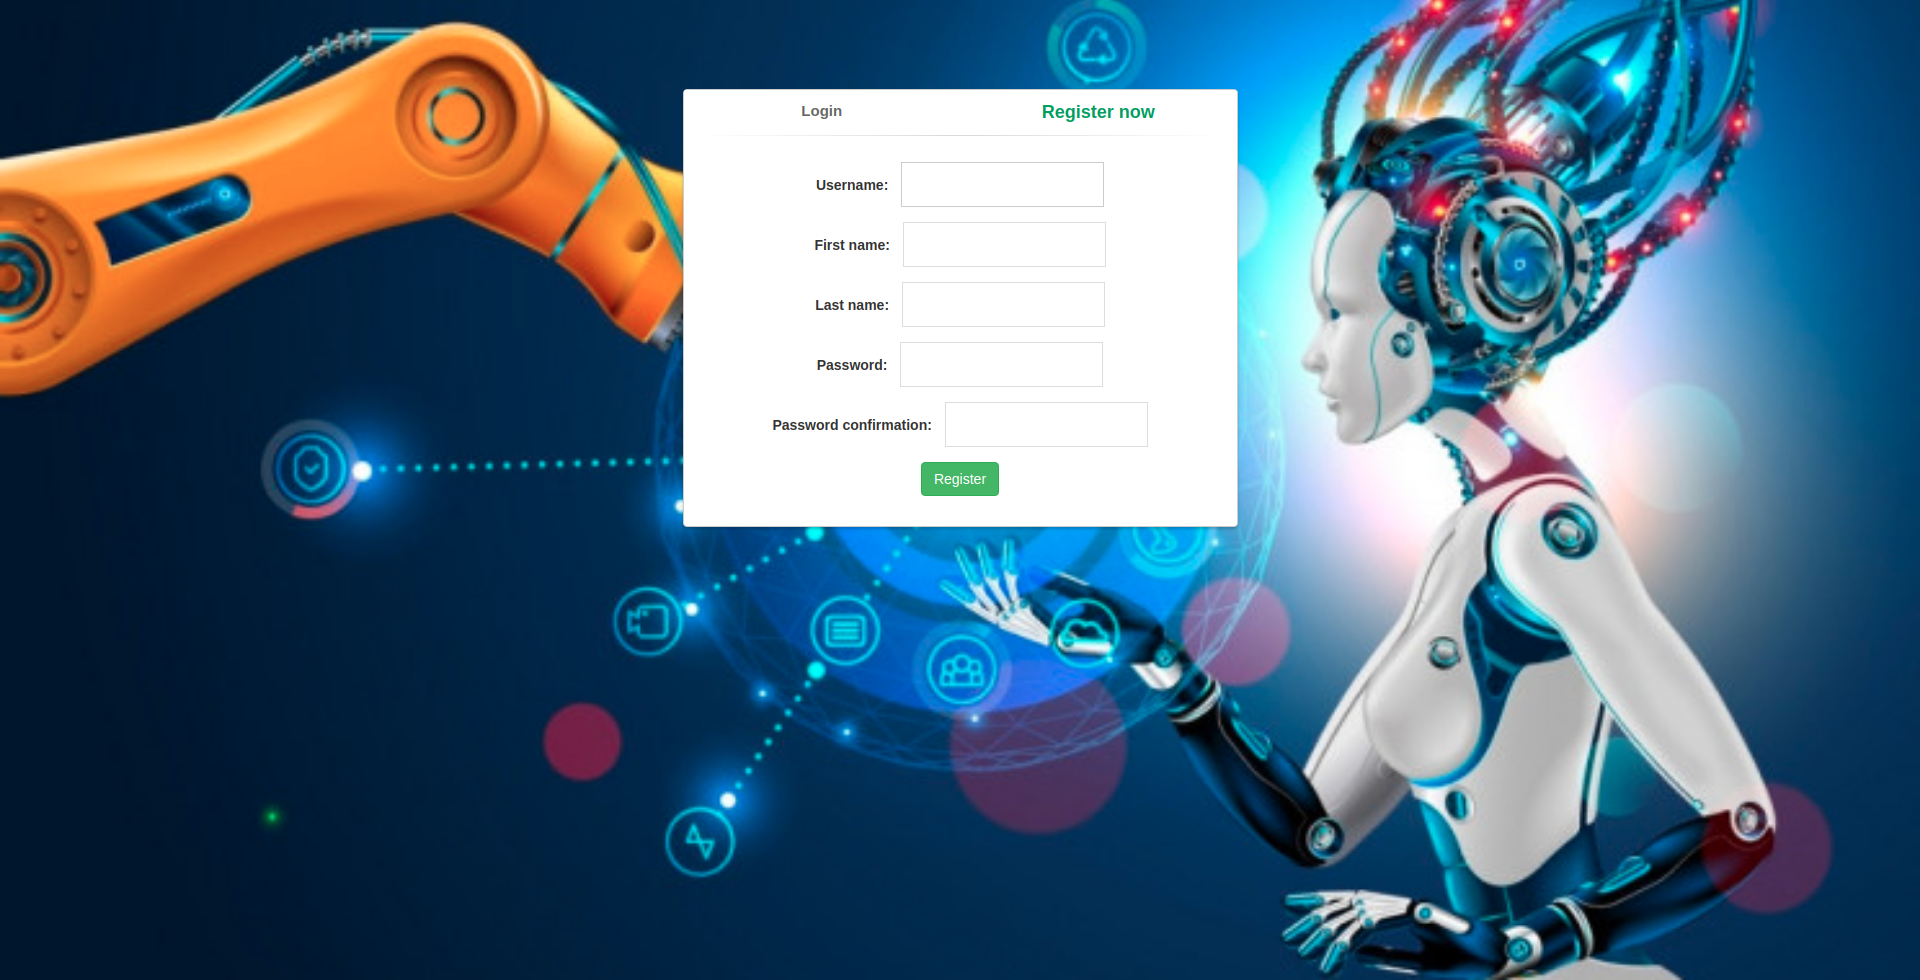
\includegraphics[scale=0.20]{images/registration_page.png}
    \caption{Registration Page.}
\end{figure}


\begin{figure}[h]
    \centering
    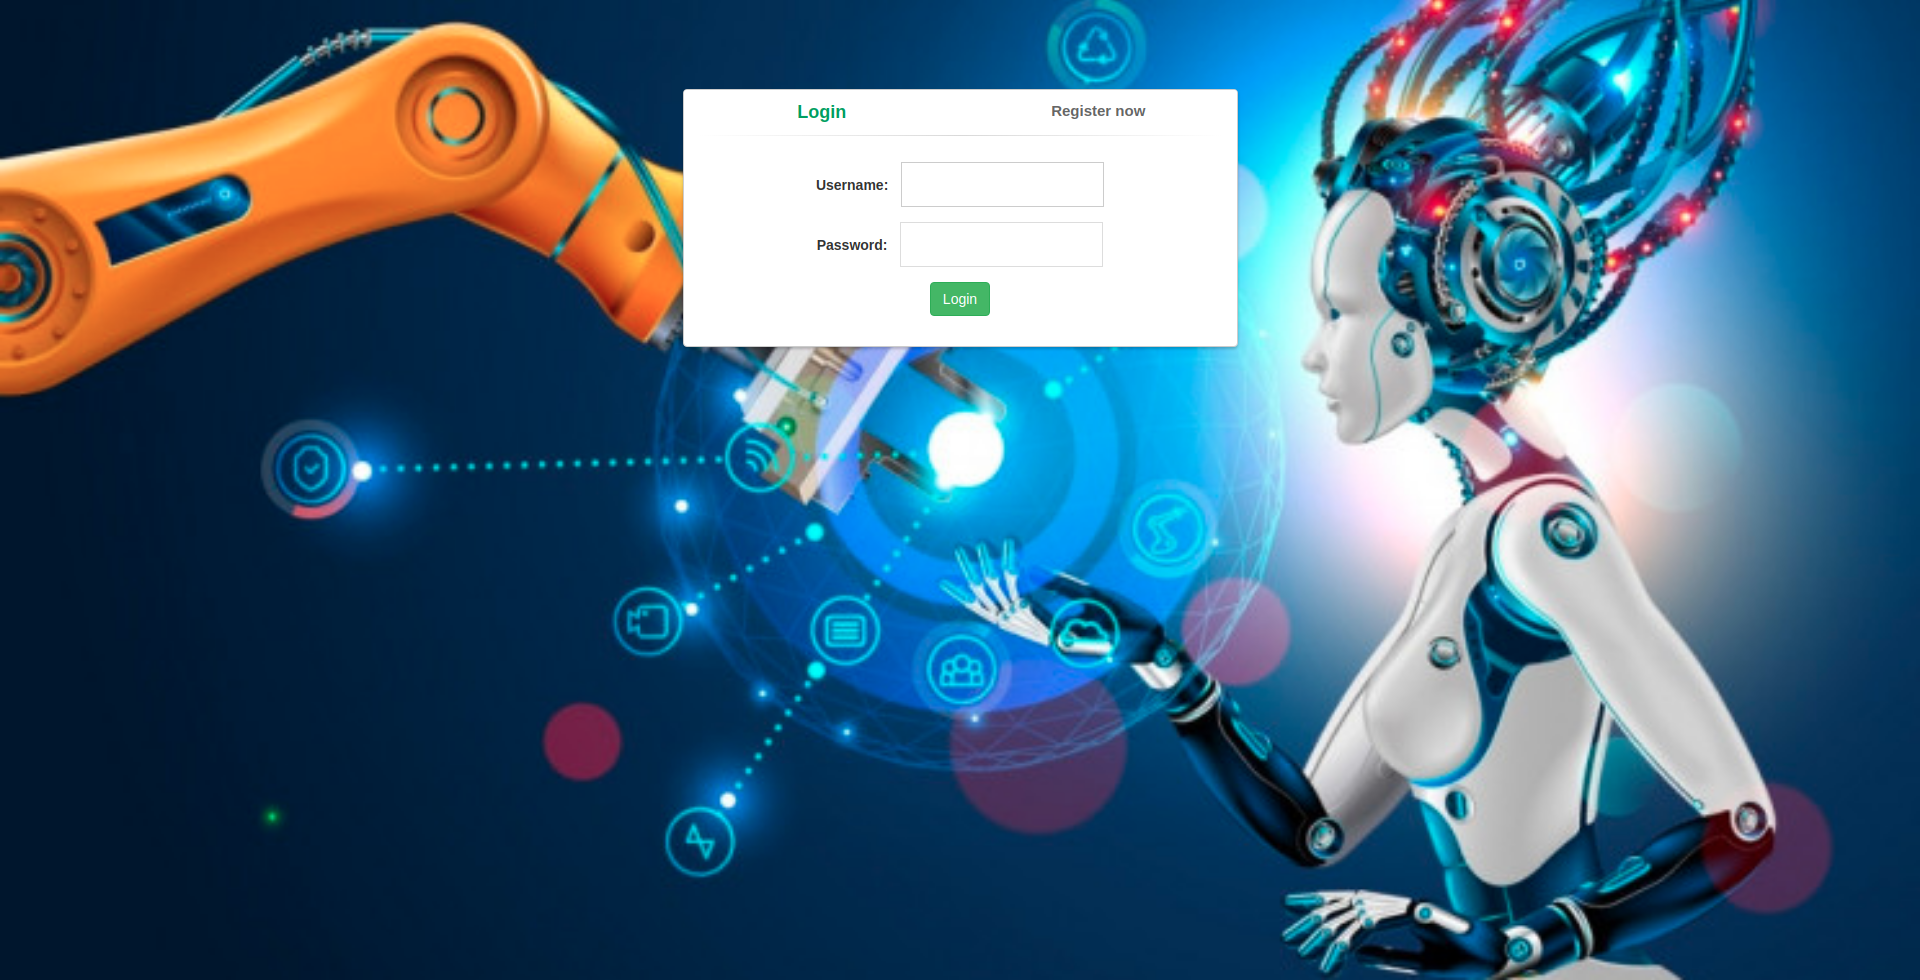
\includegraphics[scale=0.20]{images/login_page.png}
    \caption{Login Page.}
\end{figure}


\begin{figure}[h]
    \centering
    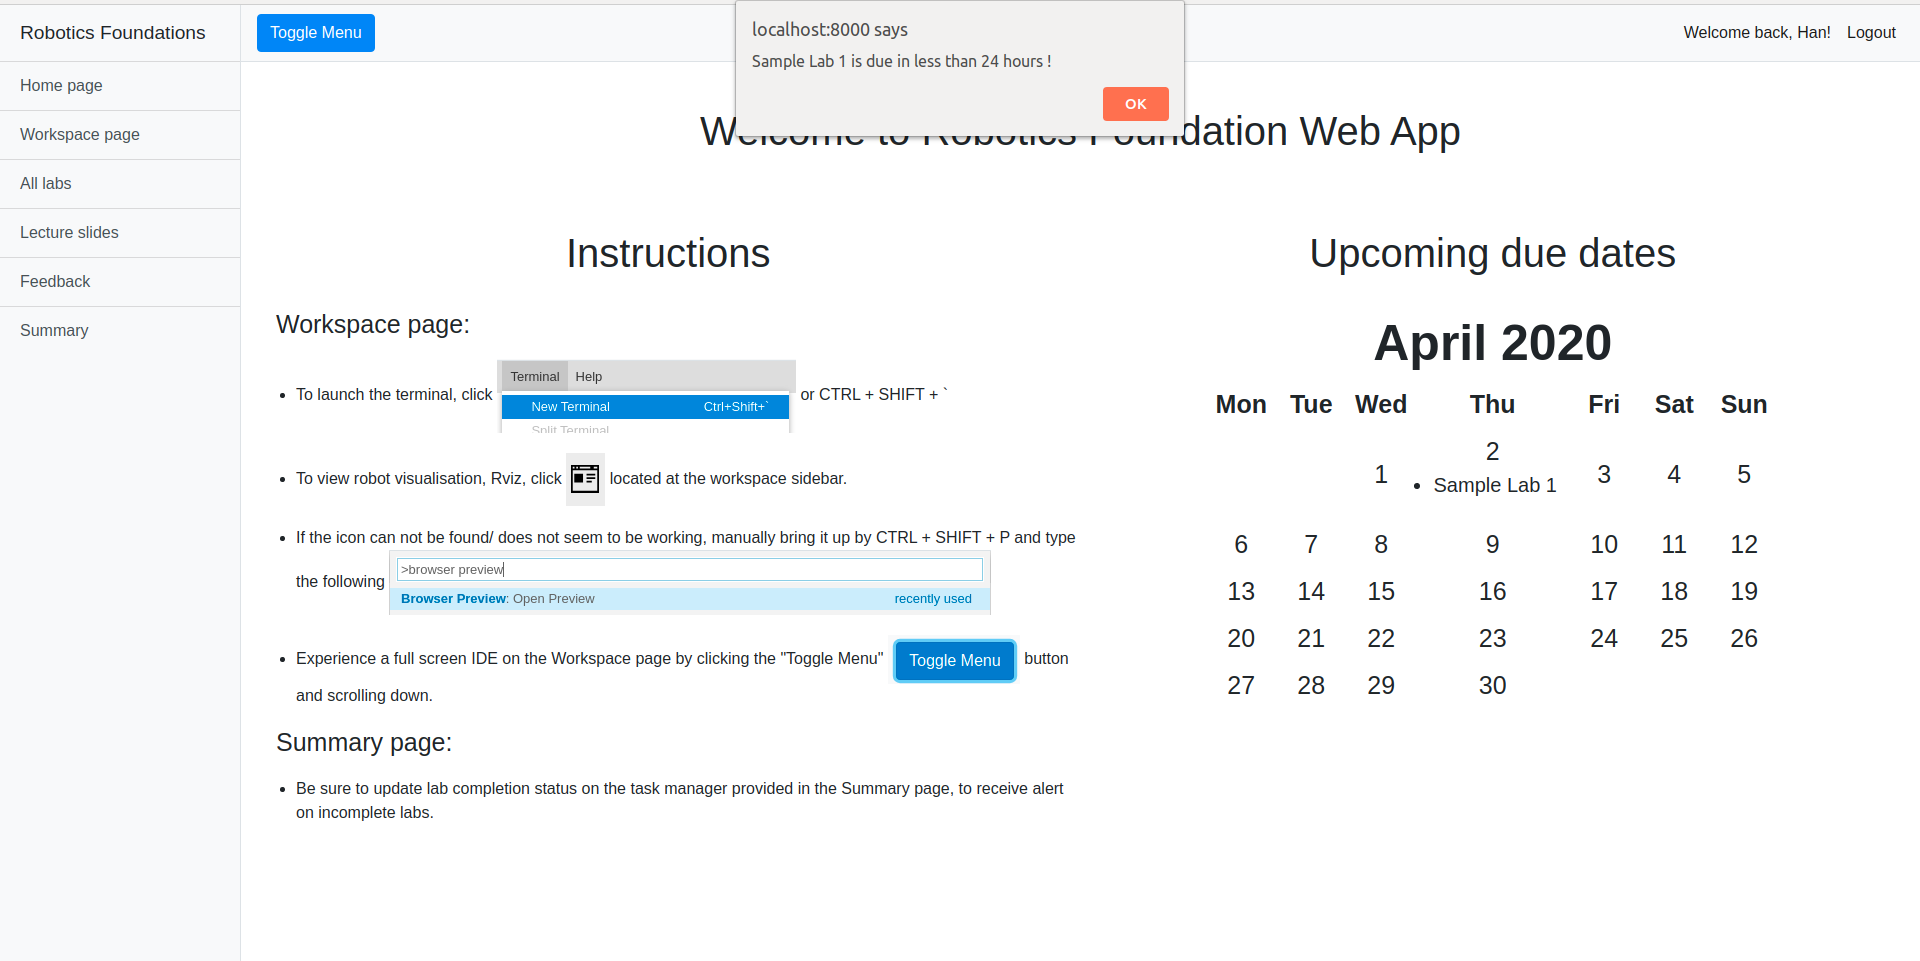
\includegraphics[scale=0.20]{images/home_page.png}
    \caption{Home Page.}
\end{figure}


\begin{figure}[h]
    \centering
    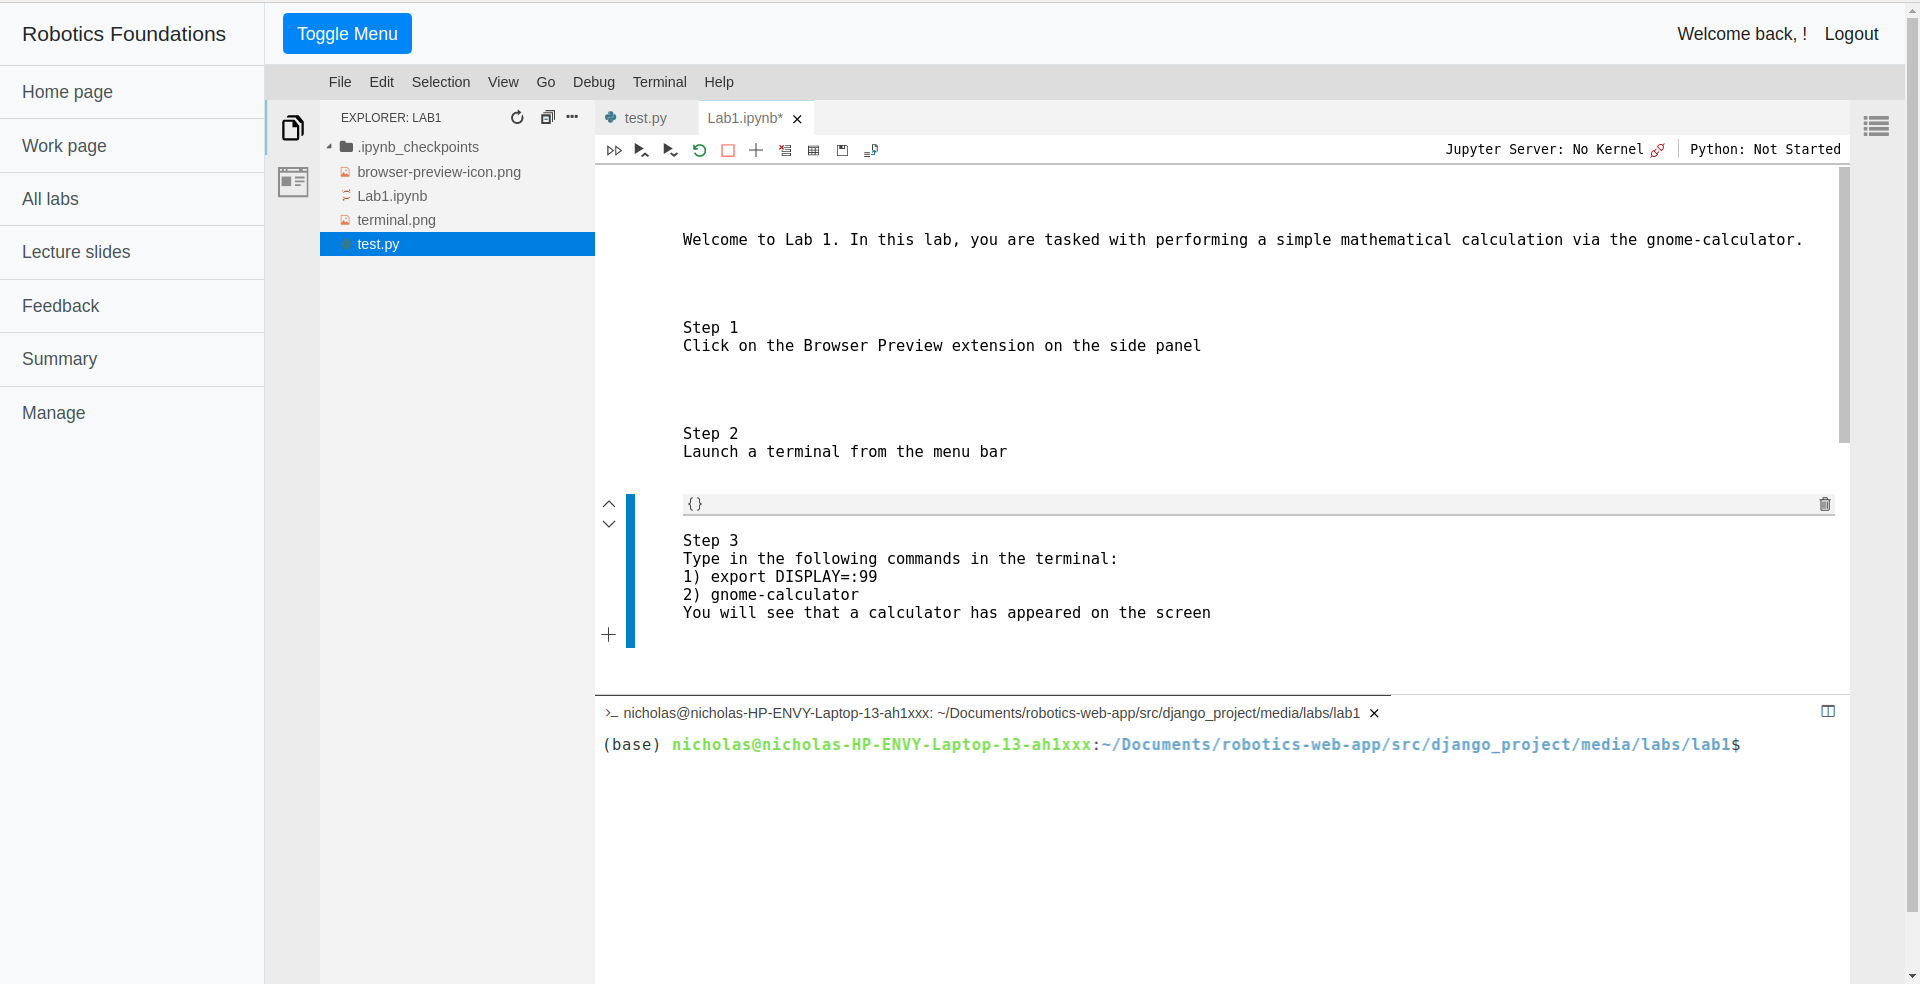
\includegraphics[scale=0.20]{images/workspace_design.png}
    \caption{Workspace Page.}
\end{figure}


\begin{figure}[h]
    \centering
    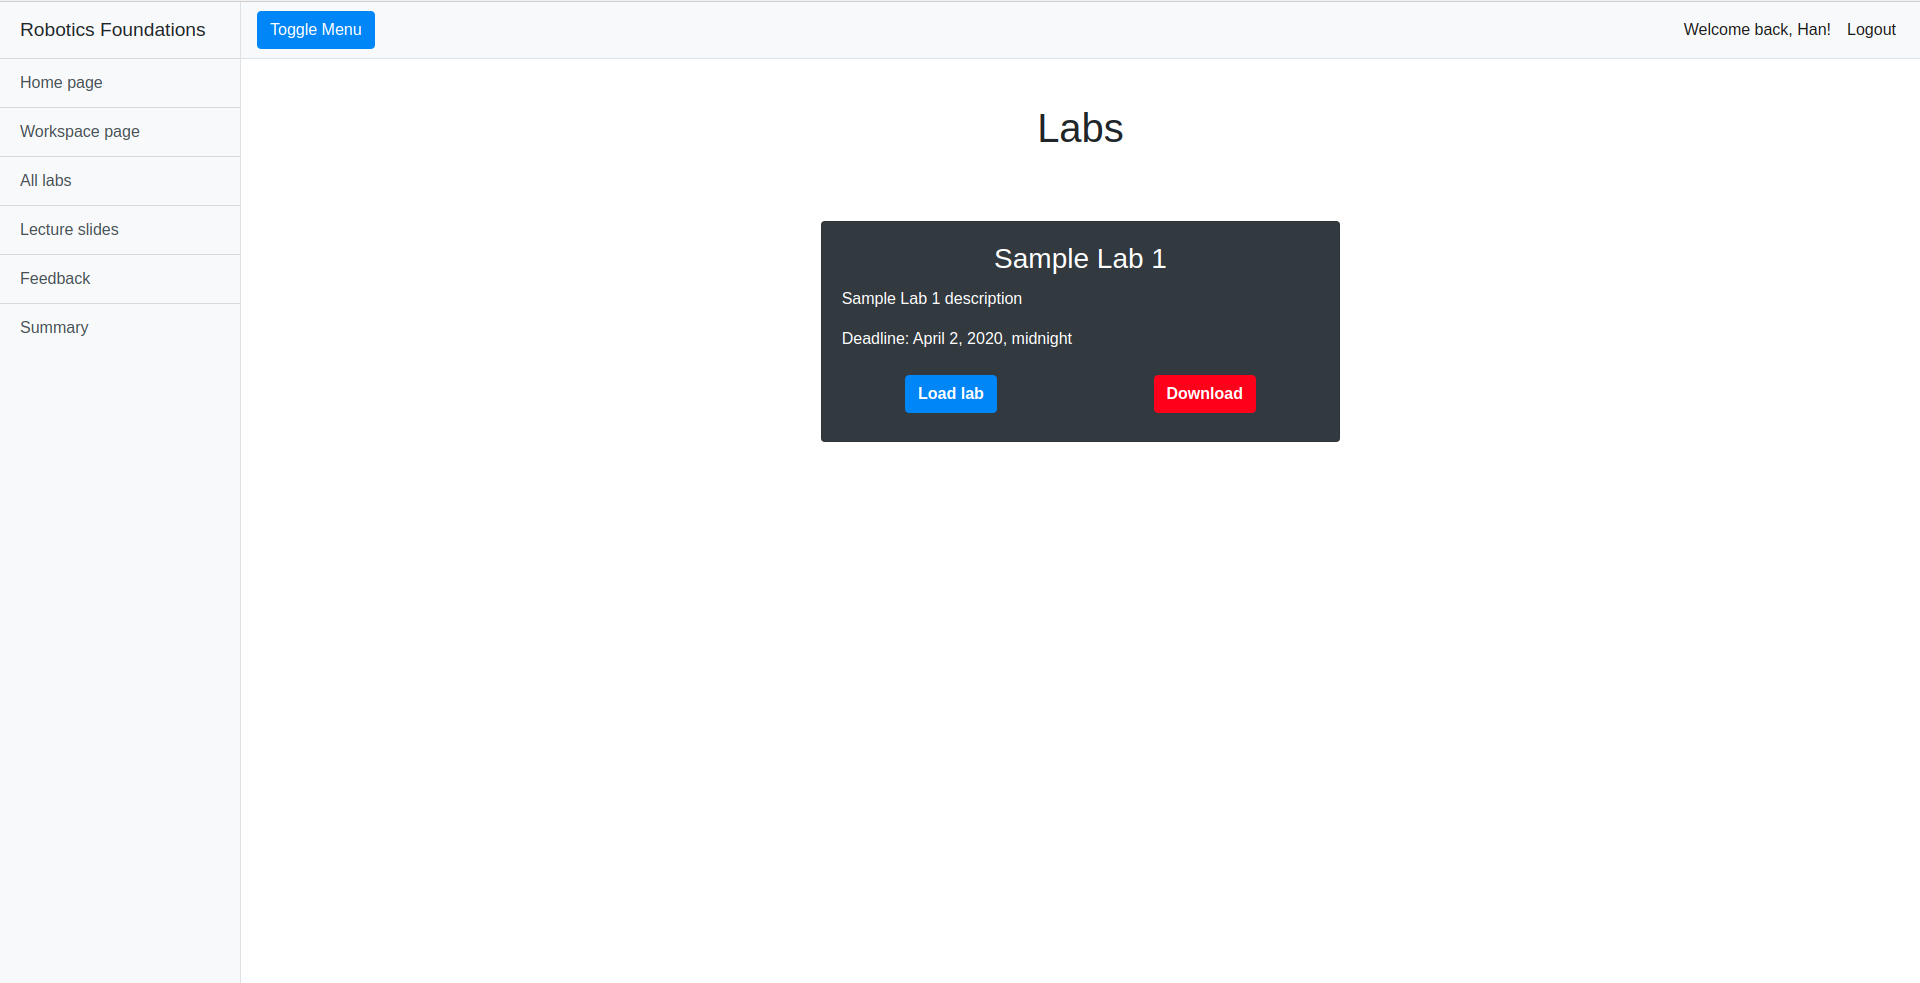
\includegraphics[scale=0.20]{images/lab_page.png}
    \caption{Labs Page.}
\end{figure}

\begin{figure}[h]
    \centering
    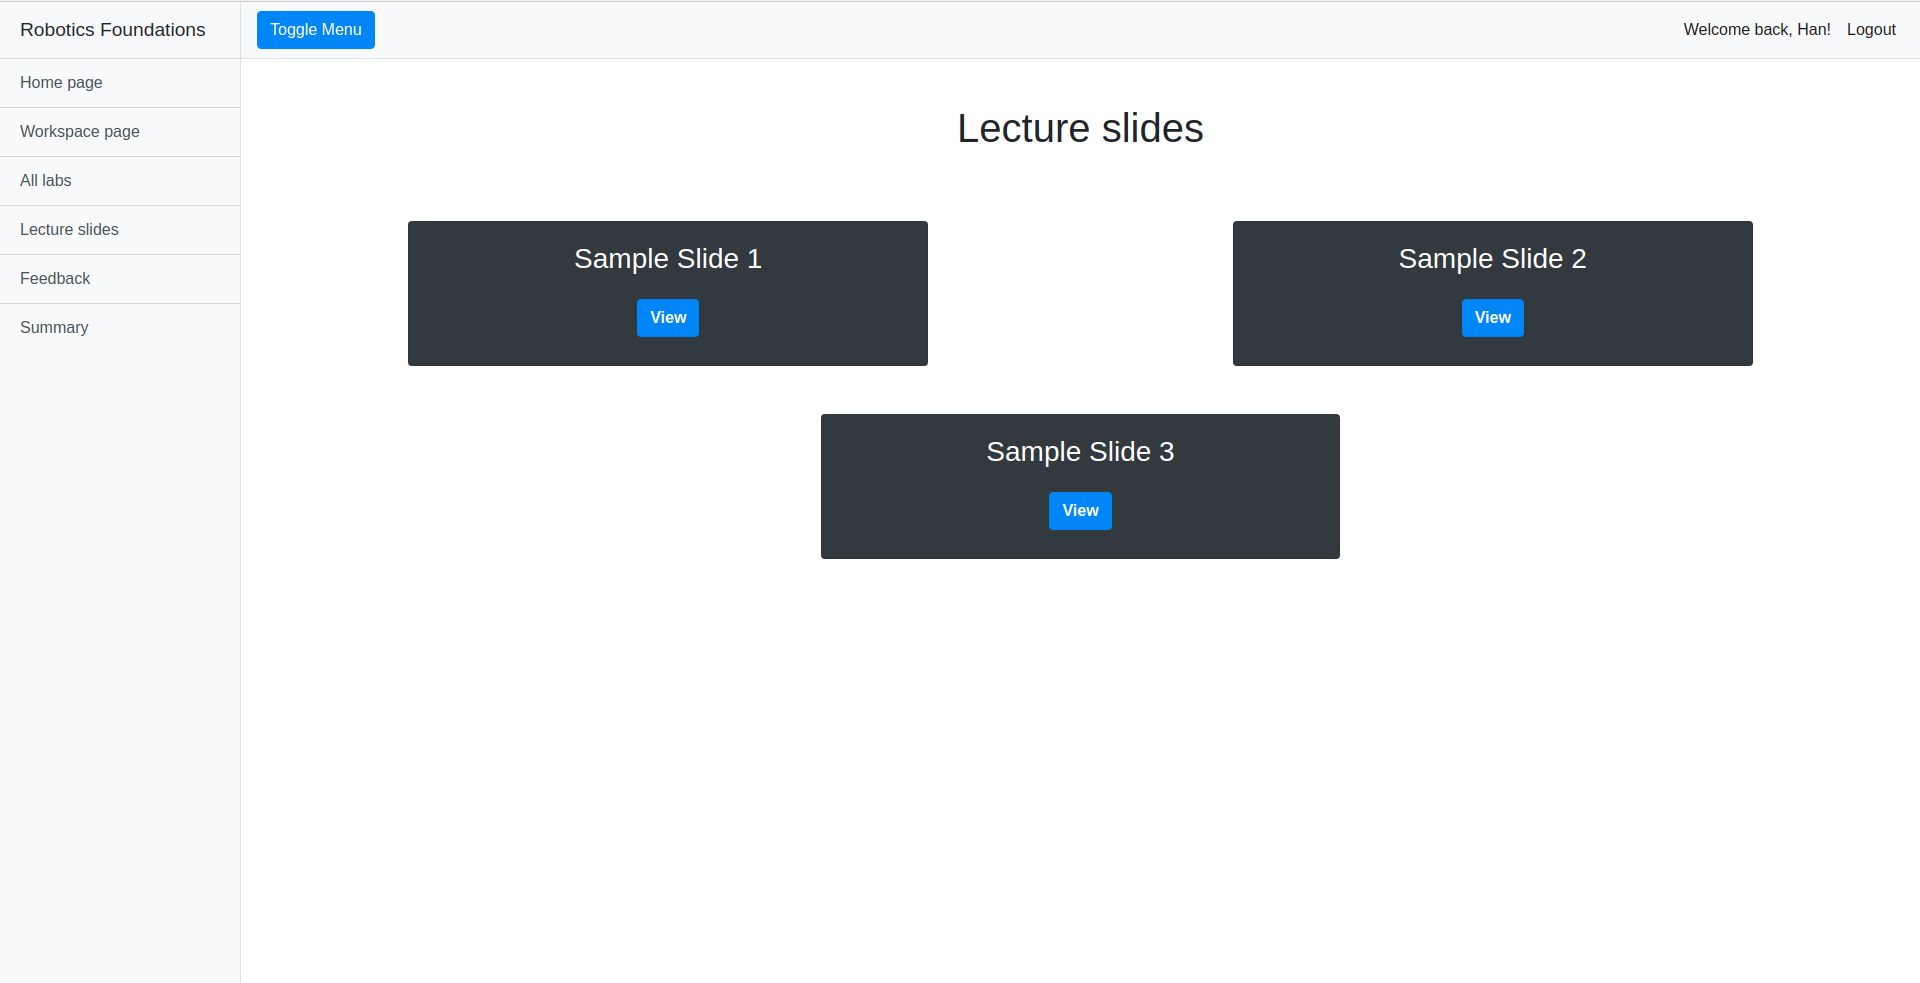
\includegraphics[scale=0.20]{images/slides_page.png}
    \caption{Lecture Slides Page.}
\end{figure}


\begin{figure}[h]
    \centering
    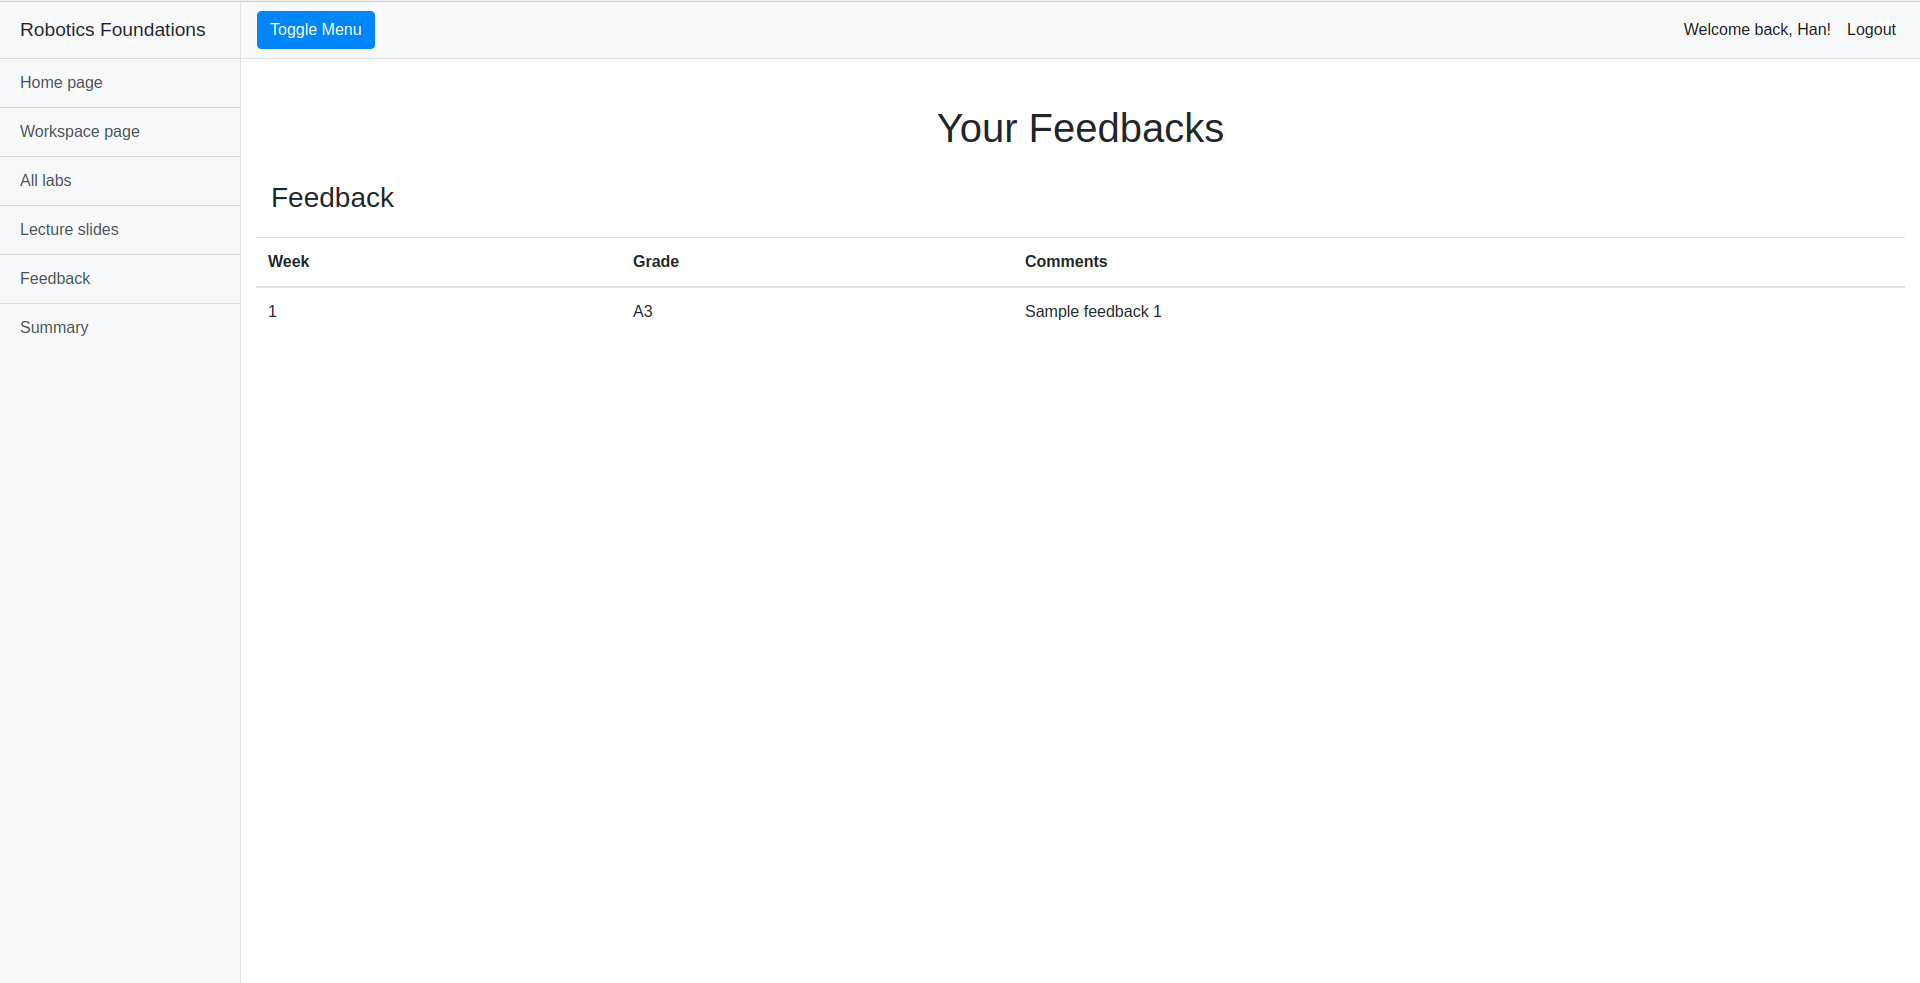
\includegraphics[scale=0.20]{images/feedback_page.png}
    \caption{Feedback Page.}
\end{figure}


\begin{figure}[h]
    \centering
    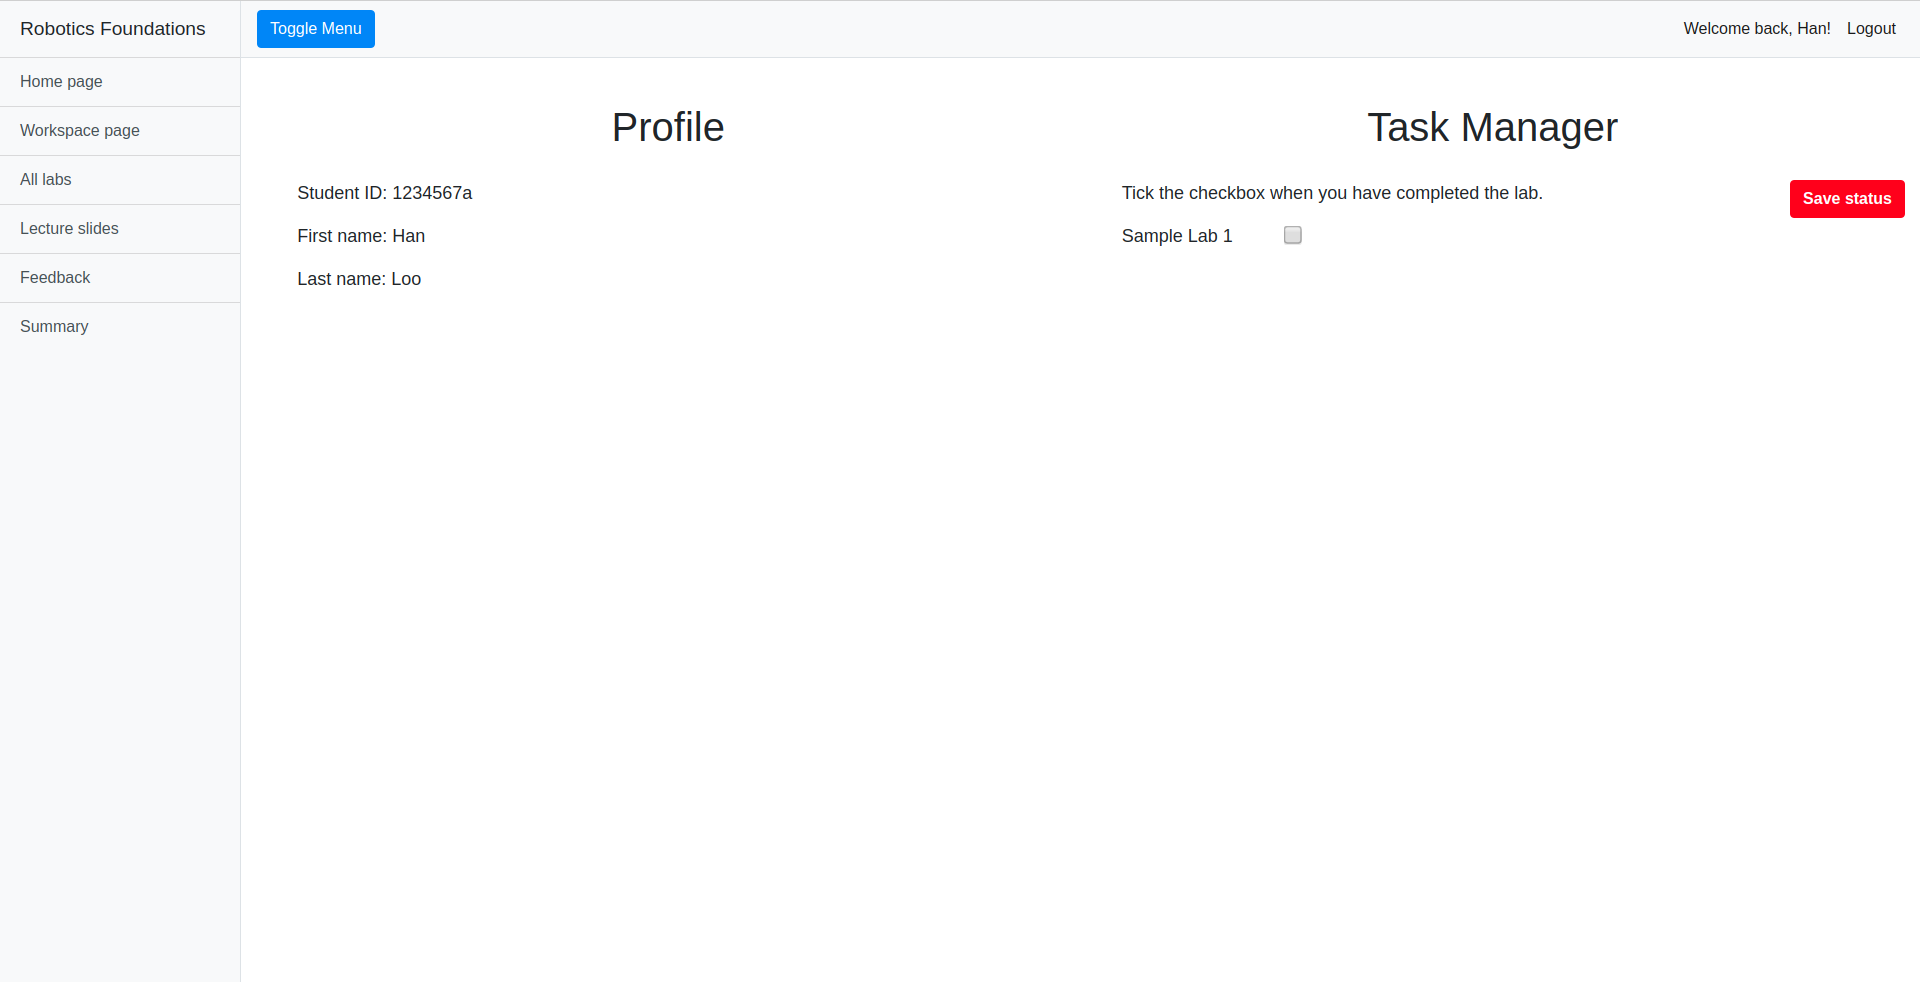
\includegraphics[scale=0.20]{images/summary_page.png}
    \caption{Summary Page.}
\end{figure}

\begin{figure}[h]
    \centering
    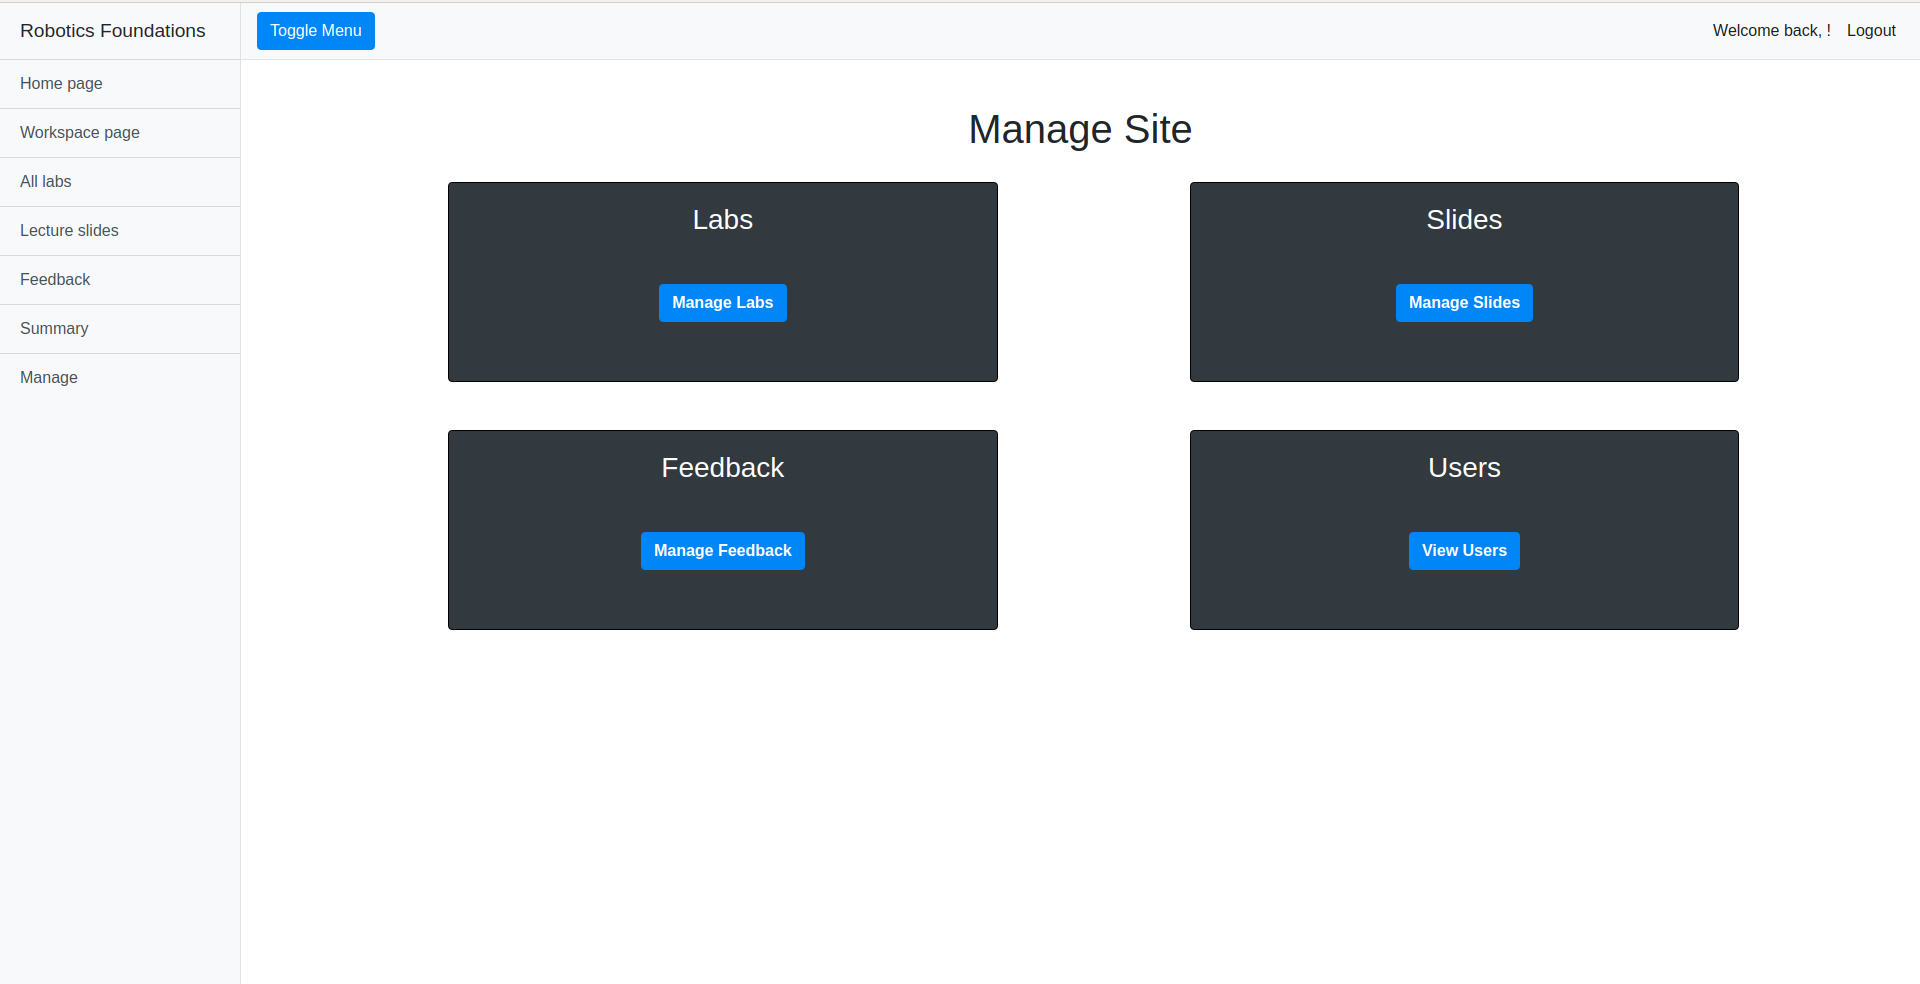
\includegraphics[scale=0.20]{images/admin_manage.png}
    \caption{Admin Management Page.}
\end{figure}

\begin{figure}[h]
    \centering
    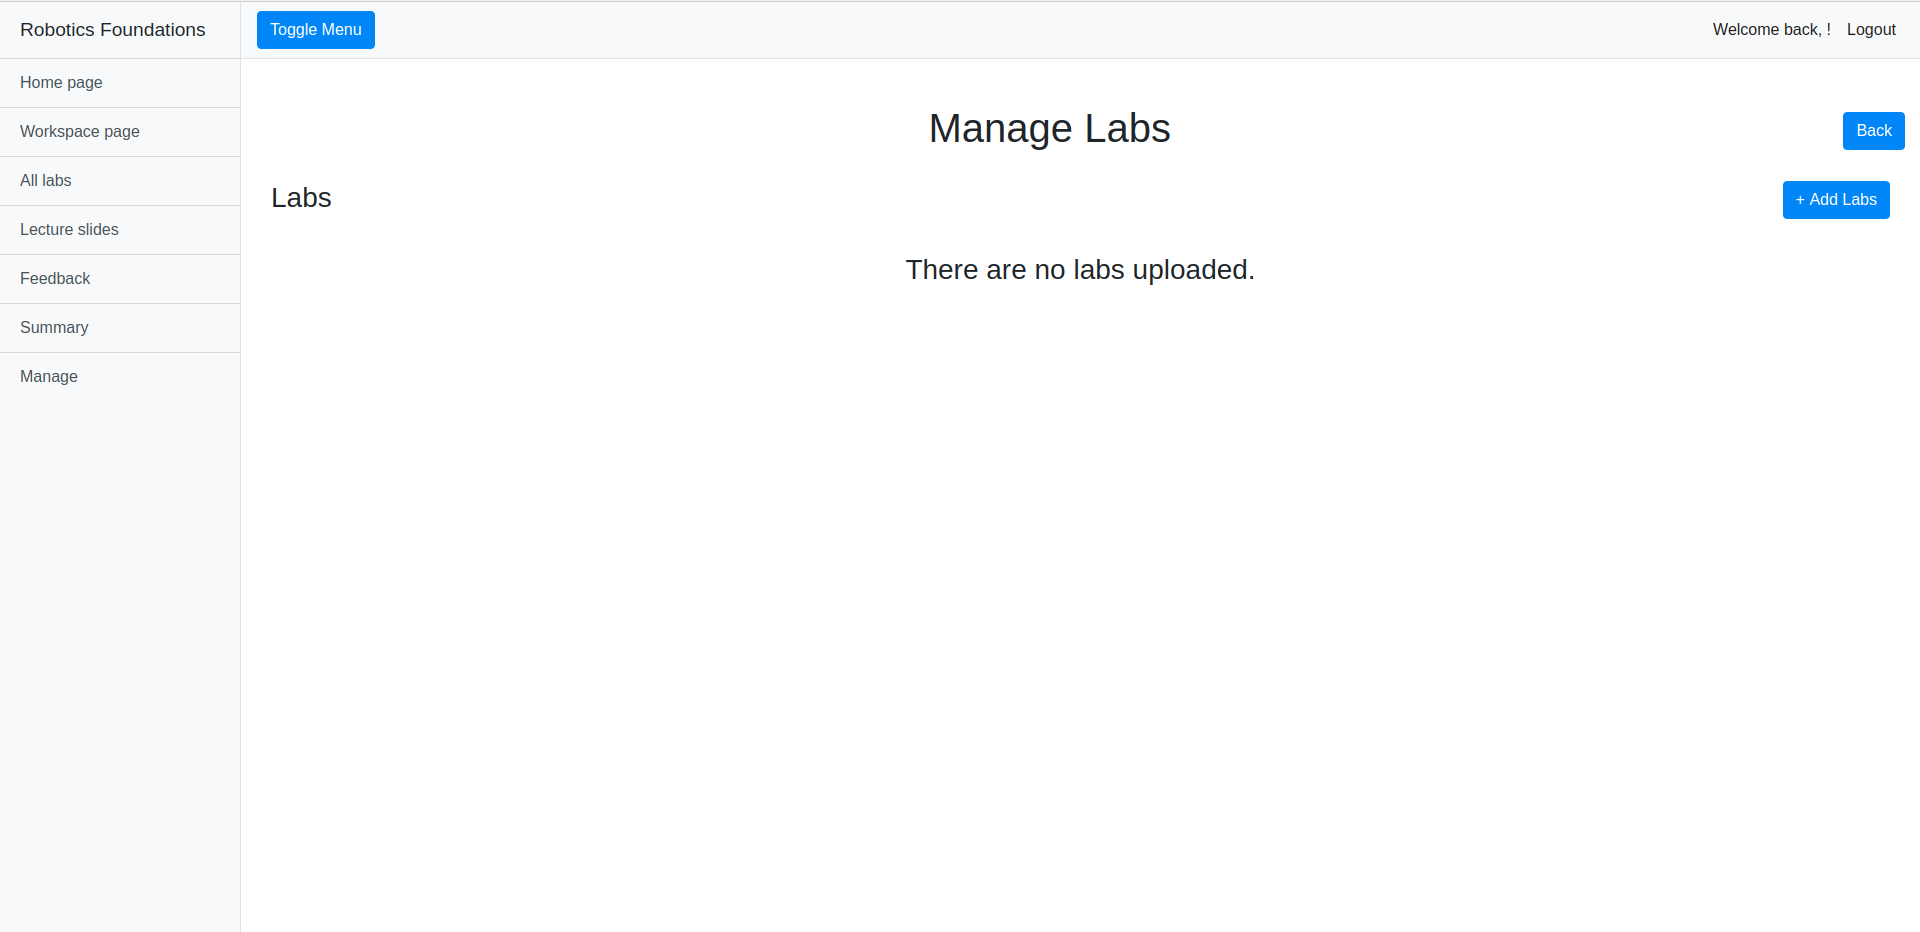
\includegraphics[scale=0.20]{images/admin_manage_lab.png}
    \caption{Admin Management Page.}
\end{figure}

\begin{figure}[h]
    \centering
    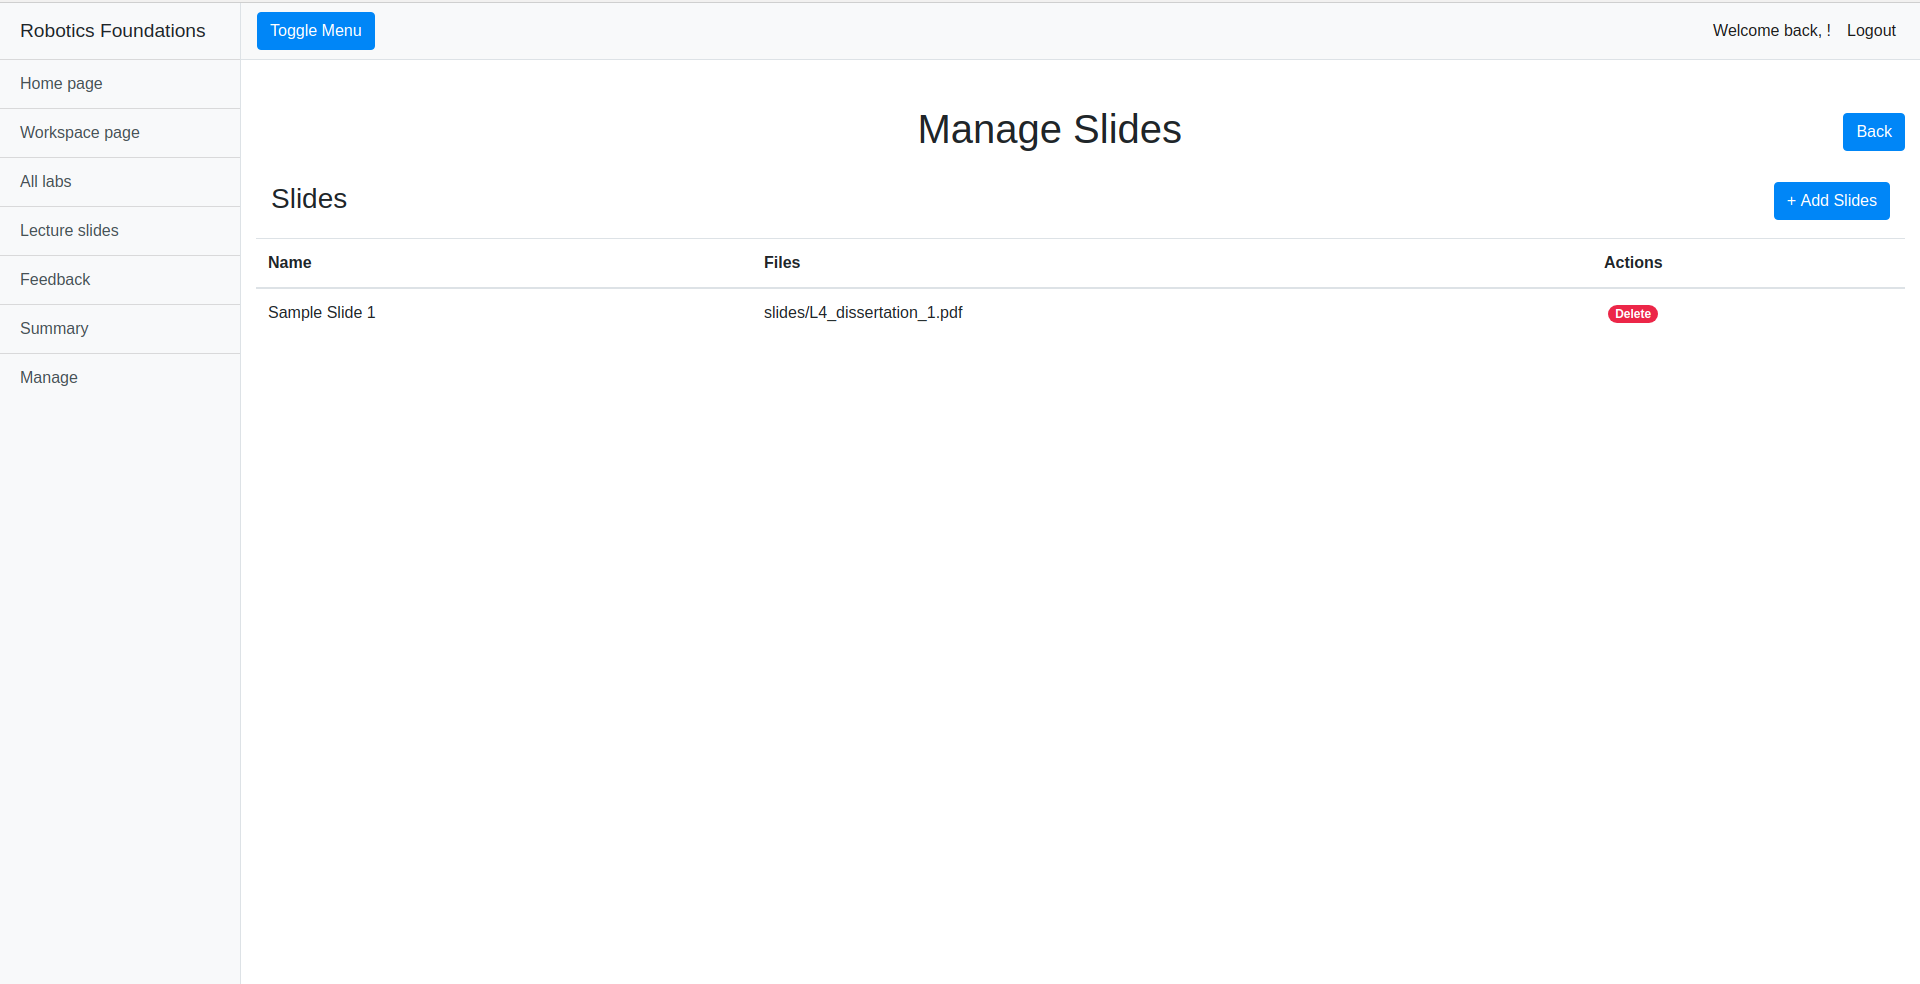
\includegraphics[scale=0.20]{images/manage_slide.png}
    \caption{Admin Management Page.}
\end{figure}

\begin{figure}[h]
    \centering
    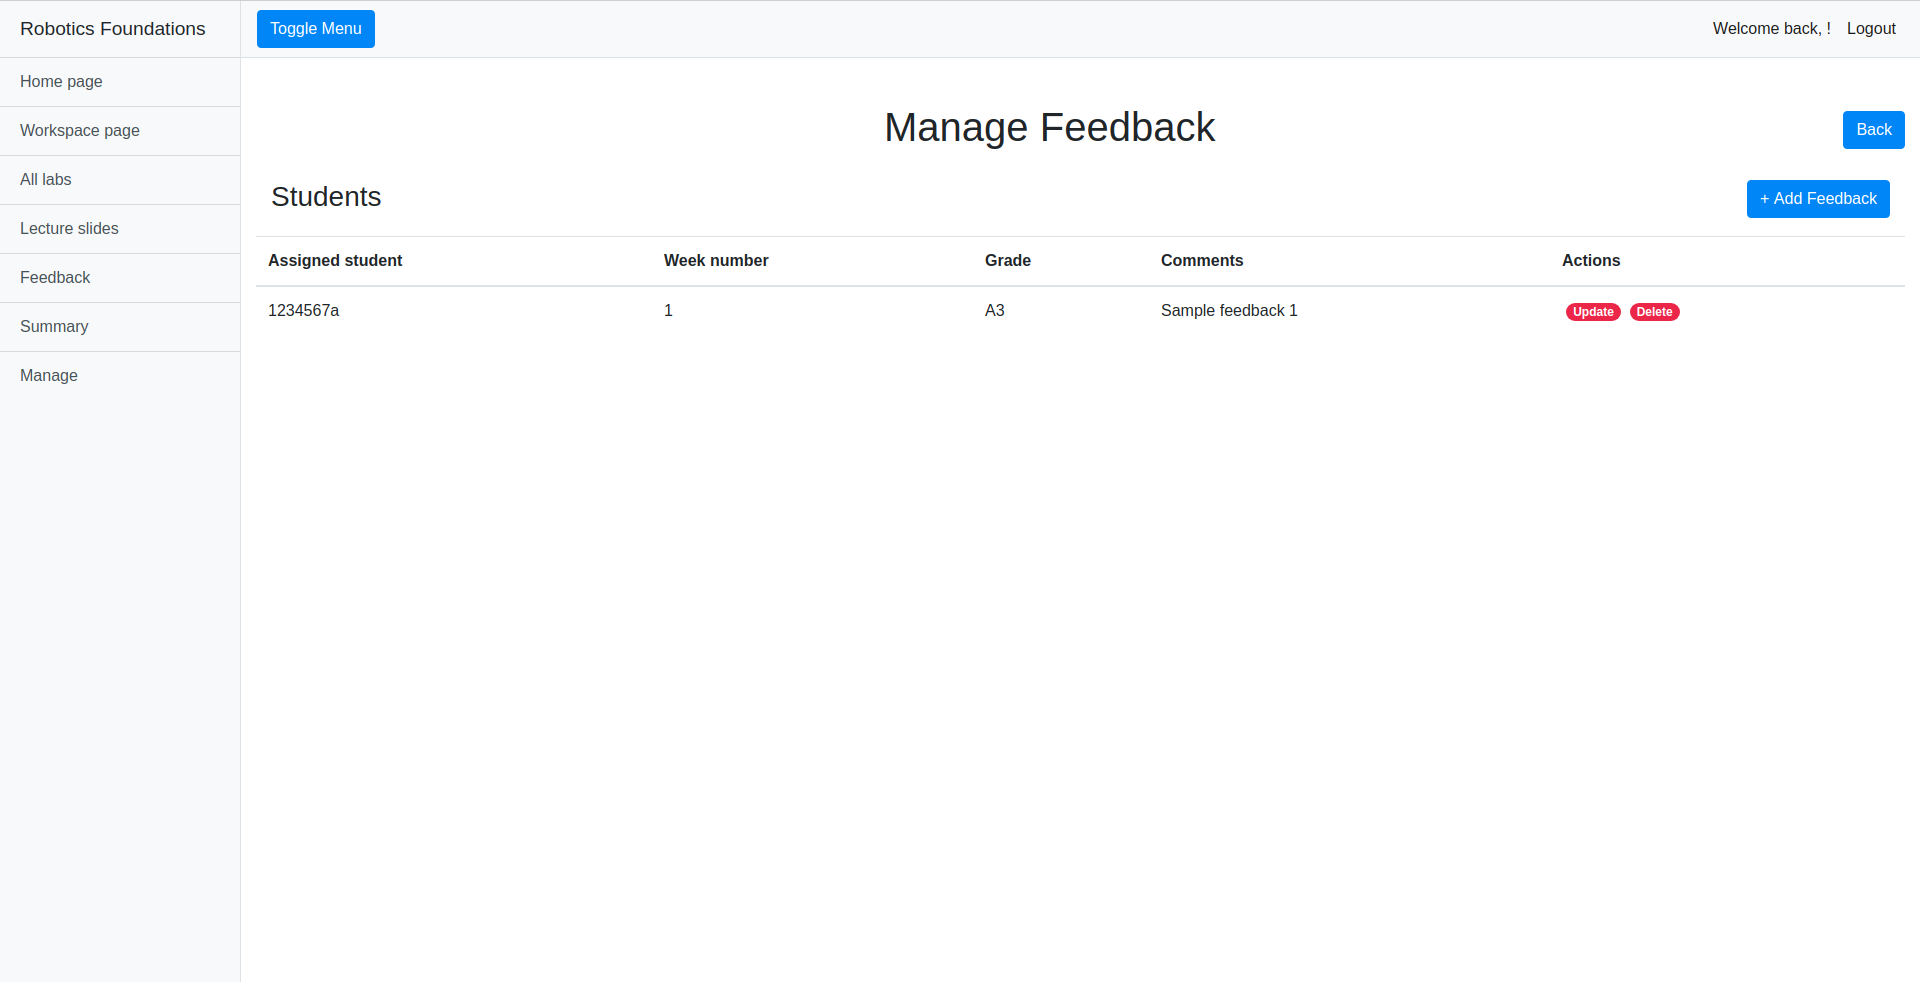
\includegraphics[scale=0.20]{images/manage_feedback.png}
    \caption{Admin Management Page.}
\end{figure}

\begin{figure}[h]
    \centering
    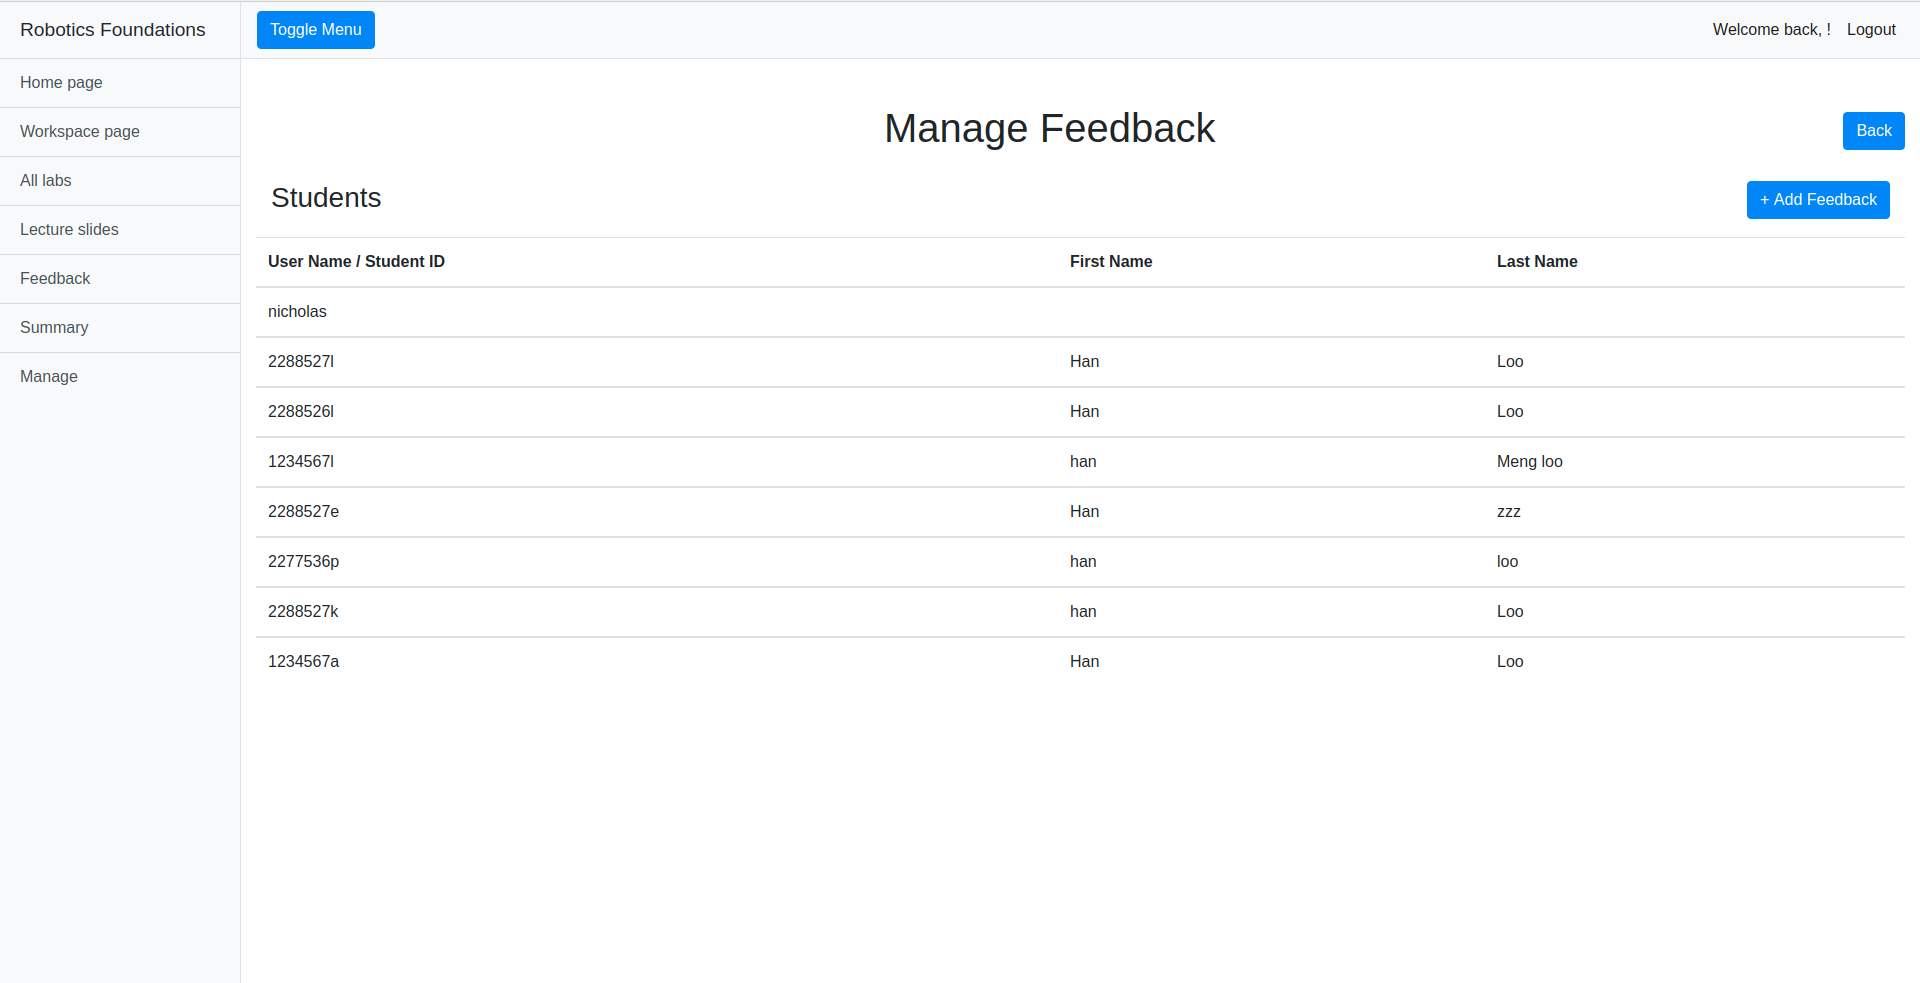
\includegraphics[scale=0.20]{images/view_users.png}
    \caption{Admin Management Page.}
\end{figure}


\end{appendices}

%==================================================================================================================================
%   BIBLIOGRAPHY   

% The bibliography style is agsm (Harvard)
% The bibliography always appears last, after the appendices.

\bibliographystyle{agsm}

% Force the bibliography not to be numbered
\renewcommand{\thechapter}{0} 
\bibliography{l4proj}

\end{document}